\documentclass[12pt]{article}
\usepackage[spanish]{babel}
\usepackage[utf8]{inputenc}
\usepackage{csquotes}

% Interlineado 1.5
\usepackage{setspace}
\onehalfspacing

% Fuente Times New Roman
\usepackage{mathptmx}

% Acomodar margenes del documento
\usepackage[a4paper, margin=2cm, top=3cm, headheight=50pt]{geometry}

% Paquetes comunes
\usepackage{graphicx, float}
\usepackage{amsfonts, amssymb, amsmath}
\usepackage{physics}
\usepackage{enumerate}
\usepackage[colorlinks=true, citecolor=blue]{hyperref}

% Para graficar
\usepackage{pgfplots}
\usepackage{tikz, color}
\usepackage{tikz-3dplot}
\pgfplotsset{width=15cm, compat=1.12}

% Para automatas
\usetikzlibrary{automata, positioning, arrows, calc, fit, babel}
\tikzset{
  automata/.style={
	->,  % makes the edges directed
	>=stealth, % makes the arrow heads bold
	shorten >=2pt, shorten <=2pt, % shorten the arrow
	node distance=3cm, % specifies the minimum distance between two nodes. Change if n
	every state/.style={draw=blue!55,very thick,fill=blue!20}, % sets the properties for each ’state’ n
	initial text=$ $, % sets the text that appears on the start arrow
  }
}

% Encabezados
\usepackage{fancyhdr}
\pagestyle{fancy}
\fancyhf{}
\fancyfoot[C]{\thepage}
\fancyhead[L]{
  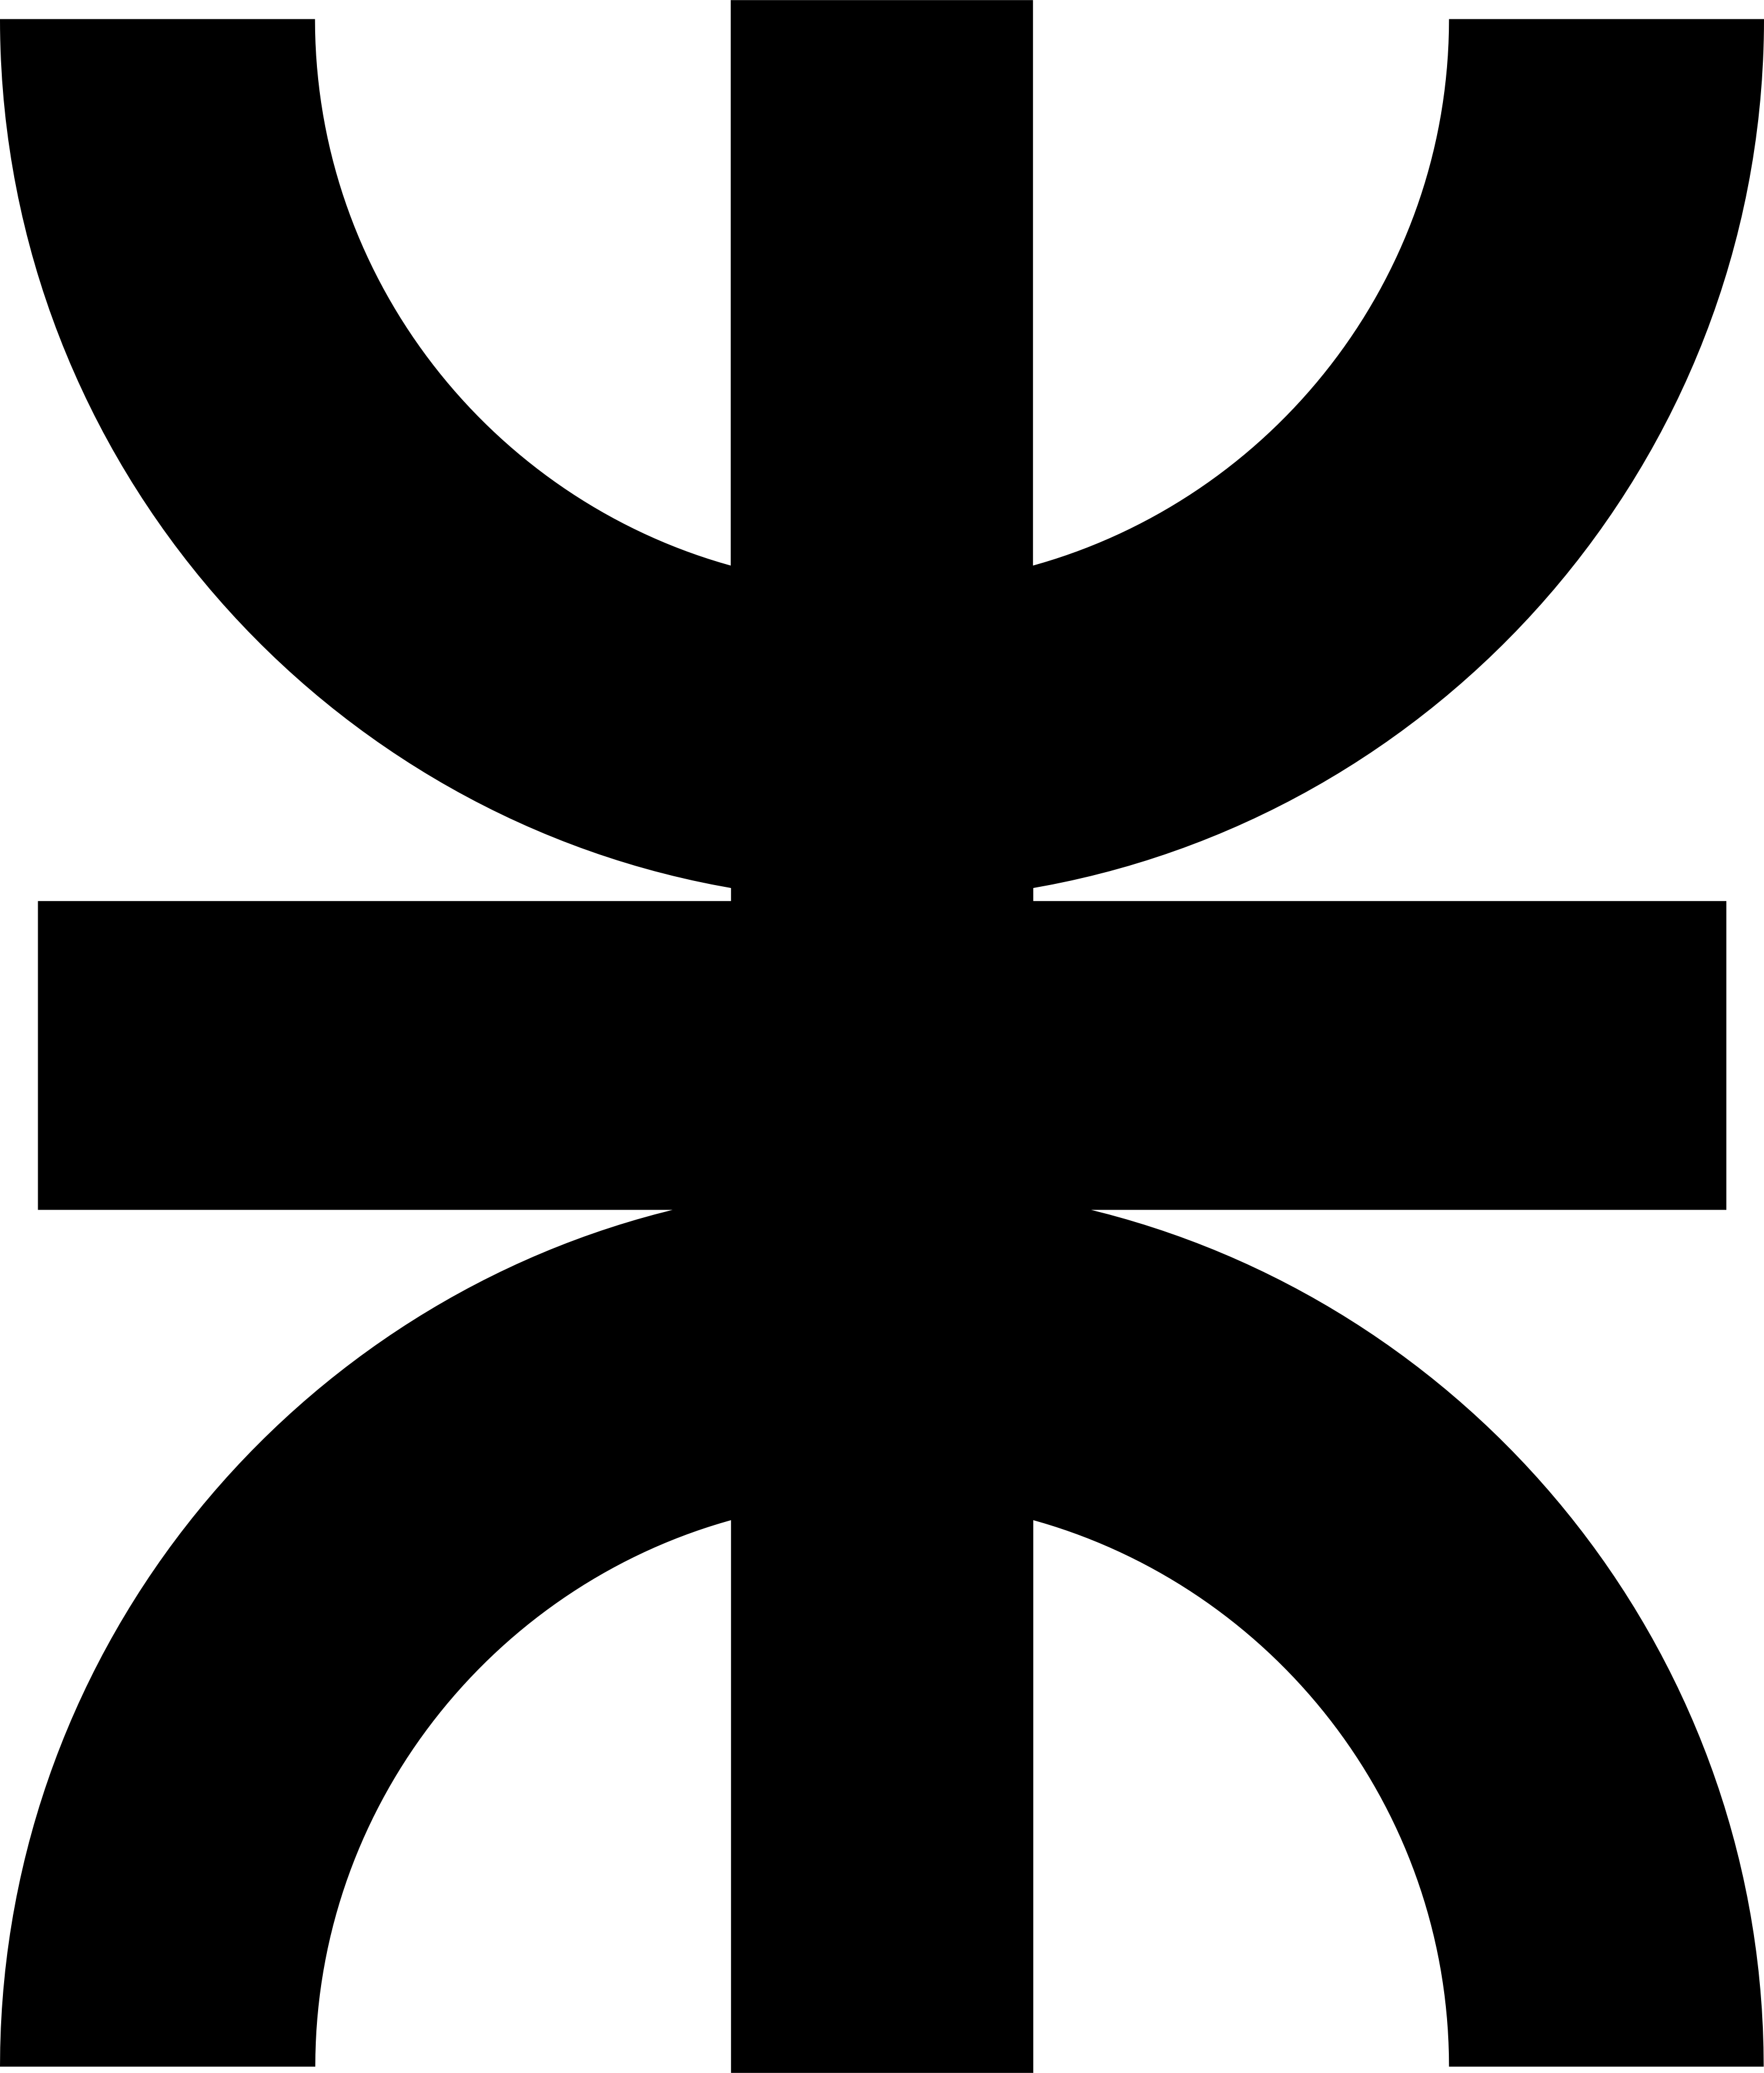
\includegraphics[height=1.2cm]{~/imagenes/logo_utn.png}
  \shortstack[l]{
    {\footnotesize Universidad Tecnológica Nacional} \\
    {\footnotesize Facultad Regional Córdoba} \\
    {\footnotesize Extensión Áulica Bariloche}
  }
}
\fancyhead[C]{
  \shortstack[c]{
    {\footnotesize Sintáxis y Semántica de los Lenguajes} \\
    {\footnotesize Resumen de la Materia} \\
    {\footnotesize }
  }
}
\fancyhead[R]{
  \shortstack[r]{
    {\footnotesize Profesor: Santiago Oliva} \\
    {\footnotesize Alumno: Ricardo Nicolás Freccero} \\
    {\footnotesize Fecha: 01/05/2025}
  }
}

% Para bibliografía
%\usepackage[backend=biber, style=apa]{biblatex}
%\addbibresource{bibliografia.bib}

\begin{document}
\newgeometry{margin=2cm, top=1.5cm}
\begin{titlepage}
	\centering
	
\includegraphics[width=\linewidth]{~/imagenes/logo_utn_frc.jpg}\\

	\textsc{
		\LARGE Universidad Tecnológica Nacional\\
		\Large Facultad Regional Córdoba - Extensión Áulica Bariloche\\
		\large Ingeniería en Sistemas de Información\\
		Año lectivo 2025\\[0.5cm]
	}

	\rule{\linewidth}{1.0mm}\\[0.4cm]
	\Huge
	\textbf{Sintáxis y Semántica de los Lenguajes}\\
	Resumen de la Materia\\[0.2cm]
	\LARGE
	Parcial 1
	\rule{\linewidth}{1.0mm}\\
	\large
	\begin{flushleft}
		Profesor: Santiago Oliva

		Ayudante:

		Fecha: 01/05/2025
	\end{flushleft}

	\vfill
	\begin{flushright}
		Alumno: Ricardo Nicolás Freccero

		Número de legajo: 415753
	\end{flushright}
\end{titlepage}

\restoregeometry
\tableofcontents
\newpage

\section{Introducción a la Teoría de Autómatas y Lenguajes Formales}
\subsection{Gramáticas formales}
A diferencia de los lenguajes naturales (castellano, ingles, etc.), que van cambiando constantemente y pueden tener diferentes interpretaciones según los pueblos y las épocas, los lenguajes formales desarrollados a partir de gramáticas formales no admiten ninguna forma de excepción o desviación. Estos surgieron de la necesidad de comunicarse con los computadores de manera inequívoca.

\subsection{Máquinas abstractas}
Son sistemas que operan en respuesta a estímulos del exterior, adoptando \textbf{estados} y enviando una respuesta al medio exterior. La conducta de estas máquinas depende tanto del estímulo recibido, como del estado en el que se encuentra en ese momento.

\subsection{Características y formalismos de las máquinas abstractas}
\begin{itemize}
	\item Reconocen que el tiempo avanza de manera discreta

	\item Para cadad intervalo de tiempo existe un único estado de la máquina.

	\item El conjunto de los estados posibles es finito y está agrupado en un conjunto o \textit{alfabeto de estados}.

	\item Recibe información o estímulos del medio exterior por medio de una \textit{cinta de entrada}.

	\item En cada intervalo de tiempo lee un símbolo de la cinta de entrada. El conjunto de todos los símbolos que reconoce se denomina \textit{alfabeto de entrada}.

	\item Pueden actuar sobre el medio exterior imprimiendo símbolos sobre una \textit{cinta de salida}. El conjunto de símbolos que es capaz de imprimir se denomina \textit{alfabeto de salida}.

	\item Las lecturas y grabaciones en cinta son realizadas en cada intervalo de tiempo por \textit{cabezales} apropiados.

	\item La \textit{función de transición} determina las aptitudes de las máquinas. Esta función define para cada símbolo de entrada y para cada estado posible, el próximo estado a ser adoptado, el funcionamiento del cabezal (si es que el autómata lo puede controlar), y el símbolo que debe ser grabado en la cinta correspondiente.
\end{itemize}

\subsection{Jerarquía de máquinas y gramáticas}
Los autómatas finitos y la máquina de Turing representan los dos extremos de una jerarquía creciente en complejidad y capacidad. En el nivel mas bajo de la jerarquía se encuentran los autómatas finitos. A estos se le pueden ir agregando mejoras hasta llegar a la máquina de Turing, que es capaz de resolver todo problema que tenga solución y, por lo tanto, representa el límite natural de lo computable.
\begin{figure}[H]
	\centering
	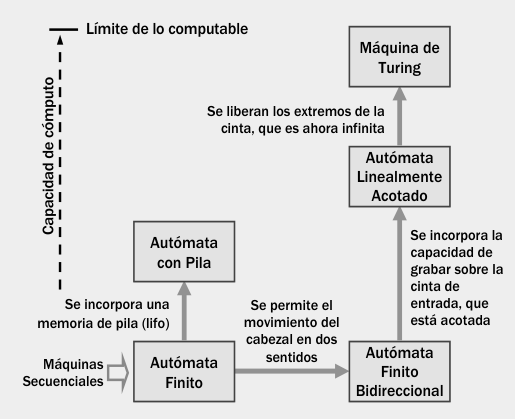
\includegraphics[width=0.7\linewidth]{imagenes/jerarquia_maquinas_abstractas.png}
	\caption{Jerarquía de las máquinas abstractas}
	\label{fig:jerarquia_maquinas}
\end{figure}

\subsubsection{Isomorfismo}
Las gramáticas formales son metalenguajes destinados a la generación de los lenguajes formales. Los autómatas son modelos de entidades reconocedoras de esos lenguajes. El lenguaje es el vínculo que establece un isomorfismo entre ambos. Esto quiere decir que el estudio de las gramáticas puede reducirse al estudio de los autómatas y viceversa. Si entendes uno, entendés el otro.
\begin{figure}[H]
	\centering
	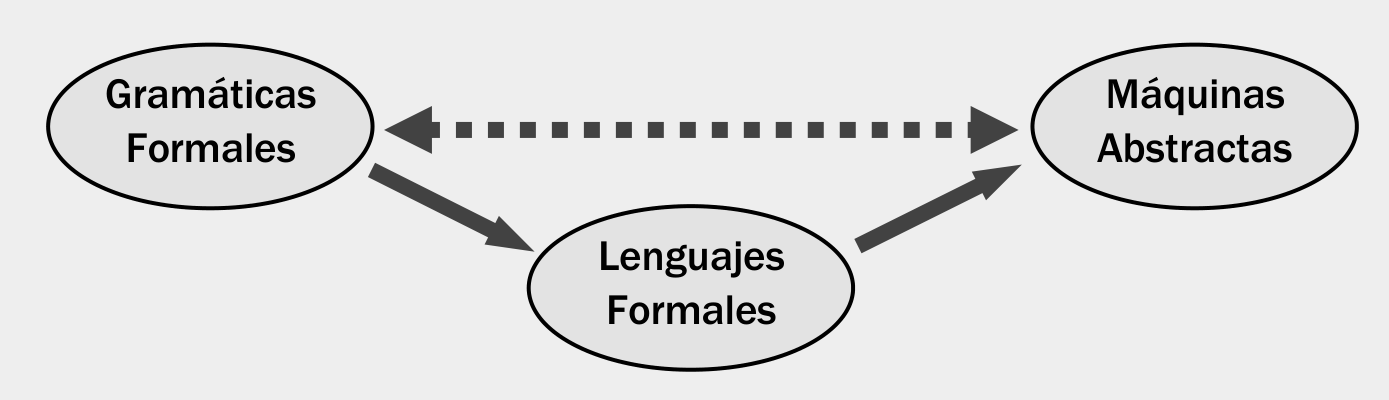
\includegraphics[width=0.7\linewidth]{imagenes/isomorfismo.png}
	\caption{Isomorfismo entre gramáticas formales y máquinas abstractas através del lenguaje formal.}
	\label{fig:isomorfismo}
\end{figure}

Chomsky clasificó las gramáticas formales en 4 tipos, de las menos restringidas a las mas, y luego a cada autómata se le asignó un nivel dentro de esa clasificación.
\begin{figure}[H]
	\centering
	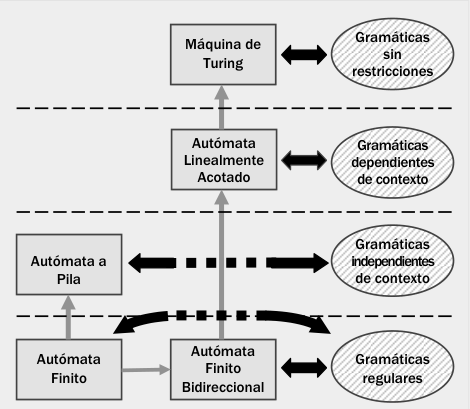
\includegraphics[width=0.7\linewidth]{imagenes/jerarquia_gramatica_maquinas.png}
	\caption{Relaciones entre las áquinas y los tipo de gramáticas según la jerarquía de Chomsky}
	\label{fig:jerarquia_gramaticas}
\end{figure}

\section{Compiladores}
Un compilador es una herramienta de desarrollo de software destinada a traducir un programa escrito en un lenguaje de alto nivel (programa fuente), en otro programa escrito en lenguaje máquina (programa objeto).

Los compiladores nacieron porque, cuando recién se habían creado las computadoras, la forma que había para programar en ellas era con códigos binarios que representaban las instrucciones individuales reconocidas por la CPU. Estos eran los \textbf{\textit{Lenguajes de primera Generación}} y su utilización era dificil y muy susceptible a errores.

Después aparecieron los \textbf{\textit{Lenguajes de Segunda Generación}}, que reemplazaron el código binario de máquina por nombres simbólicos. También se los conoce como \textbf{\textit{Lenguajes ensambladores}}. Estos lenguajes sí eran mucho mas faciles de usar que los anteriores, pero igual presentaban dificultades, como la necesidad de tener conocimientos muy profundos sobre la arquitectura de la máquina.

Para sustituir a los lenguajes ensambladores se crearon los \textbf{\textit{Lenguajes de Tercera Generación}} o \textbf{\textit{Lenguajes de alto nivel}}, que permitieron poder escribir código de programación independizándose de la máquina.

\subsection{Conceptos relacionados}
\begin{itemize}
	\item \textbf{Editor de programas}: Los programas fuente son archivos de texto que contienen el código expresado en un lenguaje de alto nivel.

	\item \textbf{Compilación}: Es el proceso de convertir un programa fuente en un programa objeto, para lo cual el compilador comienza por verificar la integridad y ausencia de errores del primero.

	\item \textbf{Compilación en varias pasadas}: Define la cantidad de veces que un compilador debe leer el programa fuente previo a la generación del programa objeto.

	\item \textbf{Intérprete}: Se denomina así a una herramienta o módulo que interpreta y ejecuta las sentencias de un programa funte una tras otra, sin generar un programa objeto.


	\item \textbf{Conversor Fuente-Fuente}: Tiene por finalidad la conversión de un programa fuente desde un lenguaje de alto nivel, a otro también de alto nivel. Por ejemplo, existen conversores $ C \to Java $ o $ C \to Pascal $.

	\item \textbf{Ensamblador}: Es un compilador cuyo lenguaje fuente es de segunda generación.

	\item \textbf{Depurador}: Llamado \textit{debugger}, es un módulo usado para facilitar las pruebas y eliminar errores de los programas.

	\item \textbf{Enlazador}: Llamado \textit{task builder} o \textit{linkeditor}, su objetivo es construir el programa ejecutable a partir del programa objeto, las librerías que pueda tener la aplicación y la librería del sistema operativo.
\end{itemize}

\subsection{Tipos de compiladores}
\begin{itemize}
	\item \textbf{Compilador cruzado}: Es un compilador que genera programas objeto que están destinados a ser ejecutados en computadores diferentes de aquél en el que se lo ha compilado. Por ejemplo, si armamos microcontroladores en la PC que están destinados a que los utilice un teclado o un mouse.

	\item \textbf{Autocompilador}: Es un compilador cuyo programa fuente está escrito en el mismo lenguaje que los lenguajes fuente que admite. Por ejemplo, muchos compiladores de lenguaje C están escritos en C.

	\item \textbf{Metacompilador}: Es un compilador que admite programas fuentes de distintos lenguajes.

	\item \textbf{Compilador optimizador}: Al generar el programa objeto, optimizan el programa para mejorar el rendimiento del sistema, manteniendo la funcionalidad original.

	\item \textbf{Compilador gráfico}: Son aquellos que admiten programas objeto representados en forma simbólica.

	\item \textbf{Compilador intérprete}: Son compiladores que generan los programas objeto en un lenguaje intermedio, que luego son interpretados en el momento de la ejecución.

	\item \textbf{Ambiente integrado de desarrollo (IDE)}: Son sistemas interactivos que incorporan al compilador servicios complementarios, tales como un editor de programas fuentes, facilidades para interpretar los programas y ejecutarlos paso paso o en forma parcial, identificar errores y gestionar las librerías de los proyectos. Un ejemplo es VSCode.
\end{itemize}

\subsection{Compiladores e Intérpretes}
Los intérpretes permiten leer y ejecutar los programas en forma progresiva, sin necesidad de cargar en la memoria al programa fuente completo, ni de generar en memoria el programa objeto. Se puede ejecutar el código del programa sin la necesidad de que esté completo.

Los compiladores necesitan cargar en memoria el programa fuente y generar el programa objeto. Se requiere una presentación completa y rigurosa del códgio fuente.

Todo compilador involucra tres lenguajes de programación:
\begin{enumerate}[1.]
	\item El del programa fuente que se desea compilar

	\item El del programa objeto que se desea generar

	\item El lenguaje de implantación, que es aquél en el que el propio compilador fue escrito.
\end{enumerate}

\subsection{Estructura y componentes de un compilador}
En la compilación, se distinguen dos etapas principales, que son las de análisis y de síntesis, motradas en la figura \ref{fig:estructura_compilador}. La etapa de análisis está dividida en tres fases y se encarga de dividir el programa fuente en sus elementos componentes y crear una representación intermedia del mismo. La etapa de síntesis también está dividida en tres fases y se encarga de reconstruir el programa objeto a partir de la representación intermedia generada.

\begin{figure}[H]
	\centering
	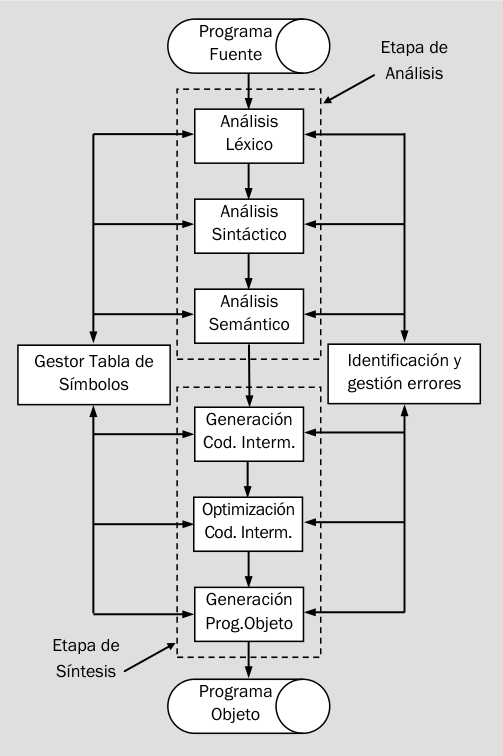
\includegraphics[width=0.4\linewidth]{imagenes/estructura_compilador.png}
	\caption{Estructura conceptual de un compilador}
	\label{fig:estructura_compilador}
\end{figure}

Vemos que a lo largo de estas etapas hay \textbf{dos módulos} esenciales que están permanentemente activos en el compilador. Uno de ellos es el módulo destinado a gestionar la Tabla de Símbolos, y el otro es el Administrador de Errores.

\subsection{Análisis léxico}
En esta fase, la cadena de caracteerers que constituye el programa fuente es leída carácter a carácter, para identificar y agrupar sus componentes léxicos. Estos componentes léxicos son secuencias de caracteres (cadenas) que tienen un siginificado colectivo y son denominados \textbf{tokens}.
En otras palabras, lo que se hace en esta fase es agarrar la cadena entera del programa fuente e identificar todas las palabras o \textbf{tokens} que hayan en la misma. Por ejemplo, si el programa era \verb|if (x==10) then return| los \textbf{tokens} generados son \verb|if|, \verb|(|, \verb|x|, \verb|==|, \verb|10|, \verb|)|, \verb|then|, \verb|return|.

\subsection{Análisis Sintáctico (Parser)}
En esta fase, se reciben las secuancias de componentes léxicos que fueron identificados en la fase anterior, y debido a que las combinaciones de estos componentes dan lugar a sentencias del programa fuente, lo que hay que hacer ahora es verificar que todas las sentencias puedan haber sido generadas por la gramática del lenguaje fuente.

\subsection{Análisis semántico}
Se revisa que la semántica de los programas fuente sea correcta. Es decir, en esta fase se detectan y comunican los errores que corresponden a:
\begin{itemize}
	\item Comprobación de tipos. Por ejemplo, que no esté sumando un entero con un caracter.

	\item Comprobación de flujos de control.

	\item Comprobación de unicidad o coherencia en las denominaciones de identificadores. Por ejemplo que no hayan dos funciones con el mismo nombre.

	\item Coherencia en los argumentos de funciones.

	\item Potenciales errores en el tiempo de ejecución. Por ejemplo cuando llamas a una función o una variable que todavía no fue declarada.
\end{itemize}

\subsection{Generación de código intermedio}
Si ninguno de los análisis anteriores tiró error, el programa fuente es convertirdo en un nuevo programa escrito en un lenguaje elemental que se denomina \textit{lenguaje intermedio}. El lenguaje universal en el que es escrito es UNCOL (Universal Compiler Oriented Language).

\subsection{Optimización de código}
Se realiza una mejora en la calidad y eficiencia del código intemedio siguiendo el siguiente orden:
\begin{enumerate}[1.]
	\item Mejoras que se refieren a la calidad de la implementación del programa desde el punto de vista lógico.

	\item Mejoras particulares para el mejor aprovechamiento global de una cierta máquina, como son la selección de las instrucciones mas apropieadas, direccionamientos, etc.
\end{enumerate}

\subsection{Generación del programa objeto}
Se toma como entrada a la representación intermedia y se produce un programa objeto equivalente, que debe ser correcto, eficiente, apropiado a la máquina en la que se va a operar y apto para dar lugar a un ejecutable compatible con el entorno (sistema operativo).

\subsection{Módulo de Gestión de Tabla de Símbolos}
Es un administrador de una tabla que contiene información sobre los identificadores del programa fuente. Esta tabla, que funciona como base de datos de la información que contiene, es definida y completada en las fases de análisis, de manera que pueda consultarse en las fases de síntesis.

En esta tabla se guardan los siguientes atributos de los identificadores:
\begin{itemize}
	\item Identidad: Si es una variable, una constante, una función, una lista, etc.

	\item Tipo: Si es un entero, un float, una string, etc.

	\item Dimensiones: En el caso de las listas.

	\item Argumentos: En el caso de las funciones.

	\item Dirección de memoria asignada.
\end{itemize}

\subsection{Módulo de Identificación y Gestión de errores}
Detecta los errores, los asocia a determinadada línea del programa fuente e intenta recuperarlo para poder seguir compilando. Cuando los compiladores están incorporados en los IDEs los errores son mostrados sobre el editor del programa fuente, facilitando la identificación y corrección por parte del programador.

\section{Gramáticas y Lenguajes Formales}
Una primera definición de lenguaje puede ser que \textit{es un conjunto de signos y de reglas que organizan esos signos}.

\subsection{Símbolos, alfabétos y palabras}
\subsubsection{Símbolos}
Un \textbf{símbolo} es un signo creado convecionalmente. Un símbolo puede ser cualquier cosa, la interpretación es lo que determina que el símbolo actúe como tal.

\subsubsection{Alfabeto}
Un \textbf{alfabeto} es cualquier conjunto finito y no vacío de símbolos. Se usan letras griegas mayúsculas para denotarlos.

Los símbolos de un alfabeto suelen llamarse también letras o caracteres.

\subsubsection{Palabra}
Una \textbf{palabra} definida sobre un alfabeto $ \Sigma $ es cualquier secuencia finita de símbolos de $ \Sigma $, escritos uno a continuación del otro. Se usan letras griegas minúsculas para denotar a las palabras.

Las palabras formadas con símbolos de algún alfabeto pueden concatenarse entre ellas para formar nuevas palabras y la concatenación se escribe como el producto de las palabras. Por ejemplo, tengo $ \alpha = casa $ y $ \beta = blanca $, entonces $ \alpha\beta = casablanca $. También existen las potencias de palabras: $ \alpha^{2} = \alpha\alpha = casacasa $.
\subsubsection{Longitud de una palabra}
Es la cantidad de símbolos que conforman una palabra y se denota como el módulo de una palabra. $ \left|\alpha\right| = 4 $

\subsubsection{Cadena vacía}
La palabra o cadena vacía se denota como $ \lambda $ y es una palabra que no tiene símbolos, por ende su longitud es cero.

\subsubsection{Potenciación de las palabras}
La potenciación está definida de la siguiente forma: \[
	\alpha^{n} = \begin{cases}
		\lambda               & , \text{si} \quad n = 0 \\
		\alpha . \alpha^{n-1} & , \text{si} \quad n > 0
	\end{cases}
\]

Existen tambien la notación $ \alpha^{-1} $ para denotar a la palabra reflejada: $ \alpha^{-1} = asac $

Aquellas palabras que son iguales a sus reflejas se denominan palíndromos.

\subsubsection{Prefijos, sufijos y subpalabras}
Supongamos que una palabra puede escribirse como una concatenación de otras tres, digamos $ \omega = \alpha\gamma\beta $; entonces decimos que $ \alpha $ es un \textbf{prefijo} de $ \omega $, $ \beta $ es un \textbf{sufijo} de $ \omega $ y $ \gamma $ es una \textbf{subpalabra} de $ \omega $. En este caso \textbf{cualquiera de las tres palabras puede ser vacía}.

De un sufijo o prefijo de una palabra se dice que es \textbf{propio} si no es la misma palabra en cuestión o la palabra vacía.
\begin{figure}[H]
	\centering
	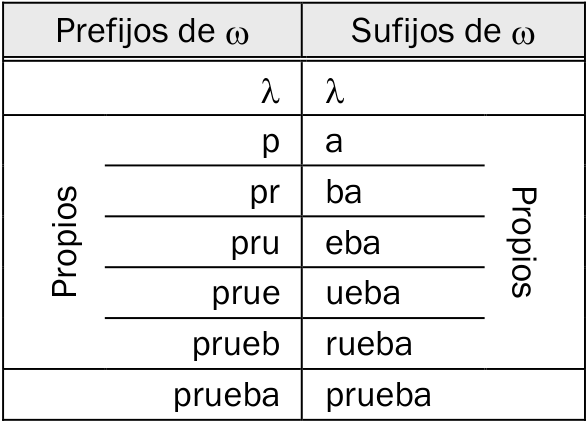
\includegraphics[width=0.4\linewidth]{imagenes/prefijos_sufijos.png}
	\caption{Prefijos y sufijos}
	\label{fig:prefijos_sufijos}
\end{figure}

\subsubsection{Operaciones con alfabetos}
Como los alfabetos son conjuntos, podemos realizar todas las operaciones que conocemos para conjuntos con ellos: los podemos unir, intersectar, restar, complementar, etc.

Podríamos operarlos con el producto cartesiano para obtener pares ordenados, pero esto no tiene mucho uso en realidad. Lo que sí podemos hacer es una operación parecida: dados dos alfabetos $ \Sigma_{1} $ y $ \Sigma_{2} $, la \textbf{concatenación} de $ \Sigma_{1} $ y $ \Sigma_{2} $, denotada como $ \Sigma_{1}\Sigma_{2} $ es el conjunto de palabras formadas por la concatenación de cada símbolo de $ \Sigma_{1} $ con cada uno de $ \Sigma_{2} $ en ese orden.

Basicamente, la operación de concatenación de dos alfabetos es lo mismo que el producto cartesiano, pero ahora en vez de generar tuplas, concatenas las letras del alfabeto.

Ejemplo:

Sean los alfabetos $ \Sigma_{1} = \left\{0,1\right\} $ y $ \Sigma_{2} = \left\{a,b,c\right\} $. Entonces:
\begin{align*}
	\Sigma_{1}\Sigma_{2} & = \left\{0a,0b,0c,1a,1b,1c\right\} \\
	\Sigma_{2}\Sigma_{1} & = \left\{a0,a1,b0,b1,c0,c1\right\}
\end{align*}

\subsubsection{Potenciación de un alfabeto}
Tomemos el alfabeto $ \Sigma_{1} = \left\{0,1\right\} $; si lo concatenamos consigo mismo obtenemos:
\[
	\Sigma_{1}\Sigma_{1} = \left\{0,1\right\}\left\{0,1\right\} = \left\{00,01,10,11\right\}
\]
que es el conjunto de todas las palabras de largo dos que pueden formarse con los símbolos 0 y 1 del alfabeto.

Se define a la \textbf{potenciación de un alfabeto} (que nos permite obtener todas las palabras de larno $ n $ del alfabeto), de la siguiente forma:
\[
	\Sigma^{n} = \begin{cases}
		\left\{\lambda\right\} & , \text{si}\quad n = 0 \\
		\Sigma\Sigma^{n-1}     & , \text{si}\quad n > 0
	\end{cases}
\]

Se denomina \textbf{universo de discurso de un alfabeto} $ \Sigma $, al conjunto de todas las palabras que pueden formarse con sus símbolos, sean del largo que sean. Este conjunto suele denotarse $ \Sigma^{*} $

El universo de disurso de un alfabeto $ \Sigma $ entonces está compuesto por todas las cadenas de símbolos de $ \Sigma $ de largo cero $ \left(\Sigma^{0}\right) $, todas las de largo uno $ \left(\Sigma^{1}\right) $, todas las de largo 2 $ \left(\Sigma^{2}\right) $, $ \dots $ y así sucesivamente.
\[
	\Sigma^{*} = \Sigma^{0}\cup \Sigma^{1}\cup \Sigma^{2}\cup \dots \cup \Sigma^{i}\cup \dots
\]

Una mejor forma de expresarlo es así:
\[
	\Sigma^{*} = \bigcup_{i=0}^{\infty} \Sigma^{i}
\]

Si al universo de discurso le quitamos la unión de la potencia cero, obtenemos el \textbf{cierre} o \textbf{clausura} del alfabeto y se denota como $ \Sigma^{+} $:
\begin{align*}
	\Sigma^{+} & = \bigcup_{i=1}^{\infty} \Sigma^{i}              \\
	\Sigma^{+} & = \bigcup_{i=0}^{\infty} \Sigma^{i} - \Sigma^{0} \\
	\Sigma^{+} & = \Sigma^{*} - \left\{\lambda\right\}
\end{align*}

El conjunto clausura de $ \Sigma $ es el conjunto de todas las palabras de largo mayor que uno.

\subsection{Lenguajes y operaciones}
Un lenguaje definido sobre un alfabeto es un conjunto de palabras construidas con los símbolos de ese alfabeto. En símbolos, si $ L $ es un lenguaje definido sobre $ \Sigma $, entonces:
\[
	L \subseteq \Sigma^{*}
\]

Como los lenguajes son conjuntos de palabras, podemos aplicar toda la teoría de conjuntos sobre ellos.

La única diferencia respecto a las operaciones que hay entre los lenguajes y los alfabetos es que en el caso de los lenguajes no podemos definir la clausura de $ L $ como la unión de todas las potencias menos la potencia 0. En símbolos, la siguiente definición es válida:
\[
	L^{+} = \bigcup_{i=1}^{\infty} L^{i}
\]
pero también es cierto lo siguiente:
\begin{align*}
	L^{+} & \neq \bigcup_{i=0}^{\infty} L^{i} - L^{0} \\
	L^{+} & \neq L^{*} - \left\{\lambda\right\}
\end{align*}

Esto se debe a que como $ L \subseteq \Sigma^{*} $, $ L $ puede contener como elemento a la cadena vacía $ \lambda $. Entonces, puede pasar que la potencia 1 de $ L $ contenga a la cadena vacía, y si se la restamos al restar la potencia 0, estaríamos perdiendo ese caracter por lo que el conjunto que tendríamos ya no sería el conjunto clausura de $ L $, porque que le faltaría un caracter que pertenece al conjunto de palabras de $ L^{1} $.

Sin embargo, siempre vamos a poder decir que:
\[
	L^{*} = L^{+}\cup \left\{\lambda\right\}
\]

\subsubsection{Descripción de los lenguajes}
Los podemos describir por \textbf{extensión} o por \textbf{comprensión}. Ya lo sabemos esto por Lógica (aguante Fabi).

\subsection{Gramáticas formales}
\subsubsection{Reglas de escritura o producciones}
Para un alfabeto $ \Sigma $ dado, diremos que una \textbf{producción} o \textbf{regla de reescritura} es un par ordenado de palabras $ \left(\alpha, \beta\right) $ definidas sobre $ \Sigma $. Las producciones las podemos ver escritas de la siguiente forma también:
\[
	\alpha := \beta
\]

Decimos que $ \alpha $ es el lado izquierdo de la producción, $ := $ es el símbolo de producción, y $ \beta $ es el lado derecho de la producción. La producción se lee \textit{alpha produce beta}.

Se llama derivación directa a la operación que aplica una sola producción a una palabra obteniendo una nueva palabra y se simboliza:\[
	\delta \to \varphi
\]

Se dice que $ \delta $ deriva directamente en $ \varphi $.

Se llama \textbf{derivación} a la operación de aplicar una secuencia finita de producciones a una cadena $ \delta $ dada para obtener otra cadena $ \varphi $, y se la simboliza:
\[
	\delta \to^{*} \varphi
\]

que se lee $ \delta $ deriva en $ \varphi $. Esto equivale a decir que existen cadenas $ \alpha_{0}, \alpha_{1}, \dots, \alpha_{n} $ tales que:
\[
	\delta = \alpha_{0} \to \alpha_{1} \to \dots \to \alpha_{n} = \varphi
\]

Si durante el proceso de derivación, cada vez que puede optarse por una producción a aplicar, se efectúa el reemplazo posible mas a la derecha en la cadena, se dice que se hizo una \textbf{derivación por derecha}. Si el reemplazo que siempre se elige es el de mas a la izquierda, se dice que se hizo una \textbf{derivación por izquierda}. Cuando las opciones se toman mezcladas, se dice que se hizo una \textbf{derivación mixta}.

Al paso contrario de la derivación, cuando vamos de una palabra derivada y llegamos a la palabra original, se dice que hicimos una \textbf{reducción}. Todo lo mismo que aplica a las derivaciones se cumple para las reducciones.

\subsubsection{Gramáticas formales}
Una gramática formal es una cuádrupla $ \left(\Sigma_{T}, \Sigma_{N}, S, P\right) $ en la cual sus cuatro componentes representan:
\begin{itemize}
  \item $ \Sigma_{T} $: es el alfabeto de los símbolos que formarán las cadenas del lenguaje que se está describiendo. Es el \textbf{alfabeto de los símbolos terminales}.

  \item $ \Sigma_{N} $: es un conjunto de variables o símbolos auxiliares llamado \textbf{alfabeto de símbolos no terminales}.

  \item $ S $: $ S\in \Sigma_{N} $ es un símbolo no terminal distinguido denominado \textbf{axioma} de la gramática.

  \item $ P $: es un \textbf{conjunto de producciones} donde ambas palabras pueden estar compuestas de símbolos terminales y no terminales, pero el lado izquiero de la producción debe tener al menos un símbolo no terminal
\end{itemize}

El alfabeto de símbolos no terminales debe ser disjunto con el alfabeto de símbolos terminales:
\[
\Sigma_{T}\cap \Sigma_{N} = \varnothing 
\]

\subsubsection{Lenguaje Generado}
Dada una gramática formal $ G = \left(\Sigma_{T}, \Sigma_{N}, S, P\right) $ se llama \textbf{lenguaje formal generado por G} al conjunto de todas las cadenas de símbolos terminales que puedan derivarse desde el axioma $ S $ usando la reglas de producción de $ P $. En símbolos:
\[
L(G) = \left\{\alpha\in \Sigma_{T}^{*}/ S\to^{*}\alpha\right\}
\]

Durante la derivacion de una cadena del lenguaje descripo por $ G $, se generarán eventualmente cadenas intermedias. Se denomina \textbf{forma sentencial} o \textbf{metapalabra} a una cadena de terminales y no terminales $ \alpha_{i}\in \left(\Sigma_{T}\cup \Sigma_{N}\right)^{*} $ que puede derivarse desde el axioma de la gramática.

La cadena final de terminales obtenida derivando desde el axioma se denomina \textbf{sentencia} o \textbf{palabra generada} por la gramática.

\subsubsection{Equivalencias de gramáticas}
Dos gramáticas $ G_{1} $ y $ G_{2} $ so \textbf{equivalentes} sí y solo sí generan exactamente el mismo lenguaje.
\[
G_{1} \equiv G_{2} \iff L(G_{1}) = L(G_{2})
\]

\subsubsection{Clasificación de las gramáticas}
Dijimos que los lenguajes formales son aquellos lenguajes que pueden ser generados por gramáticas formales. Chomsky estableció que todos los lenguajes formales podían clasificarse en cuatro tipos que solo se distinguen por el formato de las producciones de las gramáticas que lso generan. Mientras mas restricciones se le ponen a las producciones, menos lenguajes se pueden describir.

\paragraph{Tipo 0: Lenguajes estructurados por frases}\mbox{}

Son los menos restrictivos. Las producciones pueden contener cualquier cadena de terminales y no terminales tanto en lado izquierdo como en el lado derecho, con al menos un símbolo no terminal en el lado izquierdo. En símbolos:
\[
\alpha := \gamma \quad \alpha \in \left(\Sigma_{T} \cup \Sigma_{N}\right)^{*} \Sigma_{N} \left(\Sigma_{T} \cup \Sigma_{N}\right)^{*}, \quad \gamma \in \left(\Sigma_{T} \cup \Sigma_{N}\right)^{*}
\]

Donde $ \left(\Sigma_{T} \cup \Sigma_{N}\right)^{*} $ es cualquier palabra de cualquier longitud que tenga caracteres de cualquier alfabeto, y la concatencación en el medio de $ \Sigma_{N} $ nos obliga a que $ \alpha $ tenga al menos un símbolo no terminal.

\paragraph{Tipo 1: Lenguajes dependientes del contexto}\mbox{}

Son lenguajes sensibles al contexto. Sus producciones tiene la forma:
\begin{align*}
  S:= \lambda \quad \text{o} \quad \alpha A \beta := \alpha\gamma\beta \qquad \alpha,\beta \in \left(\Sigma_{T}\cup \Sigma_{N}\right)^{*}, \quad A \in \Sigma_{N}, \quad \gamma \in \left(\Sigma_{T}\cup \Sigma_{N}\right)^{+}
\end{align*}

Esto dice que el símbolo no terminal $ A $, solo puee ser reemplazado por la cadena $ \gamma $ si tiene un $ \alpha $ a su izquierda y un $ \beta $ a su derecha, es decir, \textit{si se encuentra dentro del contexto alpha-beta}.

Ademas, hay que fijarse que $ \gamma $ es una cadena que puede contener tanto caracteres terminales como no terminales, pero su longitud debe ser mayor a cero. Por esta razón, en estos casos siempre la caden del lado izquierdo es de largo igual o menor que la del lado derecho. 

Otra cosa importante es que el lenguaje podría contener como palabra a la cadena vacía, así que esta debería poder ser generada por el lenguaje. Por esto, se permite $ S:=\lambda $

\paragraph{Tipo 2: Lenguajes independientes del contexto}\mbox{}

Sus producciones pueden adoptar las siguientes formas:
\begin{align*}
  S:=\lambda \quad \text{o} \quad A:=\alpha \qquad A\in \Sigma_{N}, \quad \alpha \in \left(\Sigma_{T}\cup \Sigma_{N}\right)^{+}
\end{align*}

En este caso el símbolo terminal $ A $ puede ser reemplazado por la cadena $ \alpha $ de terminales y no terminales en cualquier lugar donde aparezca durante el proceso de derivación. Por eso estos lenguajes son \textit{independientes del contexto}.

Ademas, el lado derecho de la producción no puede ser de menor longitud que el lado izquierdo (no puede existir una \textit{regla compresora}).

Al igual que los lenguajes de tipo 1, se permite $ S:=\lambda $.

\paragraph{Tipo 3: Lenguajes regulares o lineales}\mbox{}

Las producciones tienen un solo símbolo no terminal del lado izquierdo, pero su lado derecho está compuesto por un solo símbolo terminal, o por un símbolo terminal y un no terminal, y puede contener la regla lambda.

Su formato de escritura puede ser de dos formas, totalmente equivalentes:

Regular por derecha: $ S:=\lambda \quad \text{o} \quad A:=aB \quad \text{o} \quad A:=a \qquad A,B \in \Sigma_{N}, \quad a \in \Sigma_{T} $

Regular por izquierda: $ S:=\lambda \quad \text{o} \quad A:=Ba \quad \text{o} \quad A:=a \qquad A,B \in \Sigma_{N}, \quad a \in \Sigma_{T} $

Estos formatos no pueden mezclarse en una misma gramática y seguir siendo regular (si esto pasa sería una gramática de tipo 2).

\paragraph{Tips}\mbox{}

Si en una gramática existe al menos una producción $ \alpha:=\beta $, siendo la cadena del lado izquierdo $ \alpha $ de mayor longitud que la del lado derecho $ \beta $, entonces la gramática será \textbf{tipo 0} (la regla $ S:=\lambda $ no cuenta ya que siempre es permitida). 

Si no se cumple eso, y en todas las reglas siempre un símbolo no terminal del lado izquierdo puede ser reemplazado por una cadena no vacía del lado derecho, entonces la gramática es \textbf{tipo 1}.

Si en una gramática, el lado izquierdo de todas las producciones solo tiene un símbolo no terminal, la gramátcia es \textbf{tipo 2}.

Finalmente, si todas las producciones de la gramática tienen un no terminal en el lado izquierdo y solo un terminal o un símbolo terminal y un no terminal en el lado derecho, la gramática es de \textbf{tipo 3}.

\subsection{Lenguajes regulares}
Como vimos, los lenguajes regulares son los mas restringidos en la jerarquía de Chomsky, pero ampliamente utilizados en informática. Son necesarios durante la etapa de análisis léxico de los compiladores, que tiene como tarea separar al programa fuente en tokens.

Los lenguajes regulares admiten la siguiente \textbf{definición recursiva}:
\begin{enumerate}[a)]
  \item Cualquier lenguaje \textbf{finito} $ L_{1} $ definido sobre algún alfabeto $ \Sigma $ es regular.

  \item Si $ L_{1} $ y $ L_{2} $ son lenguajes regulares, entonces también los son su unión $ L_{1} \cup L_{2} $ y su concatenación $ L_{1}L_{2} $.

  \item Si $ L_{1} $ es un lenguaje regular, entonces su estrella de Kleene $ L_{1}^{*} $ también es regular.

  \item Solo son lenguajes regulares los construidos con a), b) y c).
\end{enumerate}

\subsubsection{Expresiones regulares}\label{sec:regex}
Una expresión regular es una forma mas compacta de expresar lenguajes regulares que las gramáticas tipo 3 que vimos.

Podemos definir las expresiones regulares recursivamente como sigue:

Sea $ \Sigma $ un alfabeto, entonces:
\begin{enumerate}[a)]
  \item $ \varnothing $ es una expresión regular que denota al lenguaje vacío $ L(\varnothing ) = \varnothing  $.

  \item $ \lambda $ es una expresión regular que denota al lenguaje cuyo único elemento es la cadena vacía $ L(\lambda)=\left\{\lambda\right\} $.

  \item Cualquier símbolo $ a $ del alfabeto $ \Sigma $ es una expresión regular que denota al lenguaje cuya única palabra es la de largo unitario formada por ese símbolo $ L(a) = \left\{a\right\} $.
	  
  \underline{Si $ E $ y $ F $ son expresiones regulares, entonces: }

  \item $ E+F $ es la unión de los lenguajes denotados por $ E $ y por $ F $ $: \quad $ $ E+F = L(E) \cup L(F) $.

  \item $ EF $ es la concatenación de los lenguajes $ E $ y $ F $: \quad $ EF = L(E)L(F) $.

  \item $ E^{*} $ es el universo de discurso del lenguaje $ E $: \quad $ E^{*} = \left[L(E)\right]^{*} $.

  \item $ (E) $ es el mismo lenguaje $ E $: \quad $ (E) = E $.

  \item Solo son expresiones regulares las construidas con las pasos a) al g).
\end{enumerate}

\subsection{Lenguajes Independientes del Contexto (LIC)}
Las gramáticas independientes del contexto son muy importantes ya que describen la sintaxis de los lenguajes de programación.

\subsubsection{Gramática limpia}
Una gramática limpia es aquella que no tiene reglas o símbolos inútiles. Cuando una gramática no está limpia, hay que limpiarla para conseguir una gramática equivalente que ocupa menos espacio en memoria y su tiempo de procesamiento es menor.

Pueden existir varios tipos de  ``impurezas" dentro de una GIC, y son las siguientes:

\paragraph{Regla innecesaria}\mbox{}

Son las reglas de tipo $ A:=A $ en las que un símbolo no terminal se genera a sí mismo y no aporta nada al lenguaje. Esta regla \textbf{puede eliminarse del conjunto P} de producciones de cualquier gramática sin la necesidad de efectuar ningún cambio adicional en la misma.

\paragraph{Símbolos inaccesibles}\mbox{}

Son los símbolos terminales o no terminales de la gramática que no pueden ser alcanzados desde el axioma por ninguna derivación válida. Estos símbolos pueden ser eliminados junto con todas las producciones que los tengan y no se va a modificar el lenguaje generado.

\paragraph{Símbolo superfluo}\mbox{}

Son los símbolos no terminales que no permiten generar desde ellos al menos una cadena vacía o de solo símbolos terminales. Los símbolos superfluos junto a todas las producciones que lo contengan pueden eliminarse de la gramática y el lenguaje generado no se verá modificado. (rima :))

Ejemplo: Analicemos la siguiente gramática:
\[
G = \left(\left\{a, b\right\}, \left\{S,A,B\right\}, S, \left\{S:=aAb, A:=aAb \mid ab \mid aB, B:=aBb\right\}\right)
\]

El no terminal $ B $ resulta superfluo ya que desde $ B $ es imposible derivar una cadena de terminales. Así que lo podemos eleminar del conjunto de no terminales y quitar las dos producciones que lo contienen, obteniendo la gramática equivalente:
\[
G = \left(\left\{a,b\right\},\left\{S,A\right\},S,\left\{S:=aAb,A:=aAb \mid ab\right\}\right)
\]

\fbox{\parbox{0.9\linewidth}{
\textbf{Gramática limpia}

Se dice que una gramática independiente del contexto (GIC) \textbf{está limpia} sí y solo sí no tiene reglas innecesarias, ni símbolos inaccesibles, ni símbolos superfluos.
}}\vspace{0.2cm}

\subsubsection{Gramática bien formada}
Según la jerarquía de Chomsky, en este tipo de gramáticas no pueden existir reglas compresoras (el lado derecho de la producción es de menor longitud que el lado izquierdo). 

\paragraph{Regla no generativa}\mbox{}

Una regla del tipo $ A:=\lambda $, no siendo $ A $ el axioma de la gramática es una regla compresora denominada \textbf{regla no generativa}. Muchas veces es mejor eliminar este tipo de reglas de una gramática y para hacer eso hay que proceder de la siguiente forma:
\begin{enumerate}[a)]
  \item Para cada producción $ X:=\alpha A \beta $ que contenga el no terminal A en lado derecho, agregar regla de reescritura $ X:=\alpha\beta $ que se obtiene de reemplazar $ A $ por la cadena vacía.

  \item Luego eliminar del conjunto de producciones $ A:=\lambda $ ya que todos los efectos que produciría la misma, han sido incluidos explícitamente como producciones en el paso a).
\end{enumerate}

Por ejemplo, si tuviesemos la siguiente gramática:
\[
G = \left(\left\{a,b\right\}, \left\{S,A\right\},S,\left\{S:=aAb, A:=aAb \mid \lambda\right\}\right)
\]
, y queremos eliminar la regla no generativa $ A:=\lambda $ no podemos simplemente quitar el $ \lambda $ de las producciones de $ A $ ya que habrían cadenas que se pueden obtener estando $ \lambda $ que sin ella no se podrían obtener.

En cambio, si seguimos los pasos descriptos, la gramática quedaría de la siguiente forma:
\[
G = \left(\left\{a,b\right\}, \left\{S,A\right\},S,\left\{S:=aAb \mid ab, A:=aAb \mid ab\right\}\right)
\]
, que es una gramática equivalente a la anterior y no tiene ninguna regla no generativa.

\paragraph{Regla de redenominación}\mbox{}

Si en una gramática existen producciones del tipo $ A:=B $ donde $ A $ y $ B $ son símbolos no terminales, esta producción se llama \textbf{regla de redenominación}. Esta regla dice que $ A $ puede ser reescrito como $ B $ en cualquier contexto donde se encuentre. Sin embardo, $ A $ puede tener otras derivaciones distintas de las de $ B $ y esto puede confundir a las rutinas de análisis sintáctico.

Es necesario entonces eliminar este tipo de reglas de las gramáticas y para eso hay que seguir los pasos siguientes:
\begin{enumerate}[a)]
  \item Por cada regla $ B:=\alpha $ existente en la gramática, agregar una regla $ A:=\alpha $ para hacer explícito que a partir de $ A $ podemos derivar todas las producciones de $ B $ ($ A \to B \to \alpha $).

  \item Luego puede eliminarse $ A:=B $ del conjunto de producciones y la gramática obtenida será equivalente a la original.
\end{enumerate}

Ejemplo: Dada
\[
	G = \left(\left\{0,1\right\},\left\{S,T\right\},S,\left\{S:=0S \mid S1 \mid T, T:=01 \mid 0T\right\}\right)
\]
, para quitar la regla de redenominación $ S:=T $ seguimos los pasos anteriores.

Tenemos que agregar al conjunto de producciones de la gramática $ S:=01 $ y $ S:=0T $, que son todas las producciones de $ T $, para poder quitar la regla de redenominación. Entonces la gramática equivalente sin dicha regla queda así:
\[
G = \left(\left\{0,1\right\},\left\{S,T\right\},S,\left\{S:=0S \mid S1 \mid 01 \mid 0T, T:=01 \mid 0T\right\}\right)
\]

\fbox{\parbox{0.9\linewidth}{
\textbf{Gramática bien formada}

Se dice que una gramática independiente del contexto (GIC) está \textbf{bien formada}, sí y solo sí, está limpia y no tiene reglas no generativas ni de redenominación.
}}\vspace{0.2cm}

\subsection{Análisis sintáctico}
El análisis sintáctico es un proceso mediante el cuál podemos determinar si una cadena pertenece a un lenguaje determinado o no. Para lograr esto podemos encontrar una derivación $ S \to^{*} \alpha $, o demostrar que tal derivación no existe. Este procedimiento puede llegar a ser extremadamente largo y tedioso, por lo que se crearon métodos claros y repetibles para realizar el análisis.

\subsubsection{Árbol de derivación}
Un árbol de derivación es un árbol cuyo nodo raíz es el axioma de la gramática, cuyos hijos son todas las posibles derivaciones. Cada nodo a su vez tiene también como hijos a todas sus derivaciones de manera que todos las hojas del árbol son símbolos terminales.

Ejemplo: Supongamos que tenemos la siguiente gramática:
\[
G = \left(\left\{0,1\right\}, \left\{S,P,Q\right\}, S, \left\{S:=PQ \mid 0S1, P:=0Q \mid 1, Q:= 1P \mid 0\right\}\right)
\]
y queremos saber si la cadena $ 0101 $ pertence al lenguaje $ L(G) $. Para eso podemos partir de $ S $ e ir armando el árbol de dervación para ver si podemos conseguir la cadena $ 0101 $.
\begin{figure}[H]
  \centering
  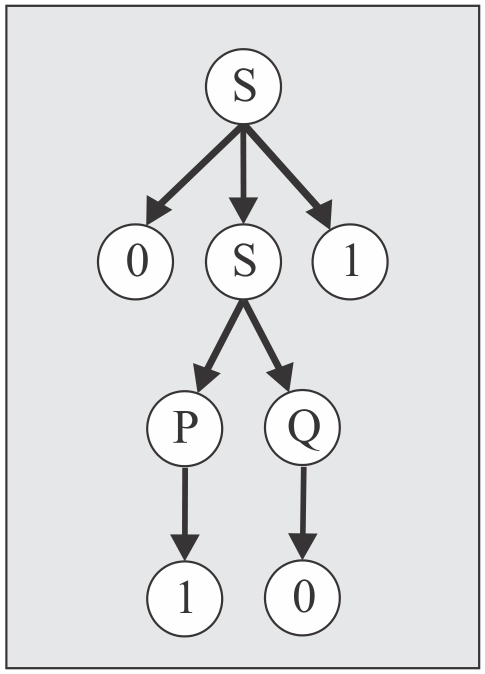
\includegraphics[width=0.3\linewidth]{imagenes/arbol_derivacion.png}
  \caption{Árbol de derivación de la cadena $ 0101 $}
  \label{fig:arbol_derivacion}
\end{figure}

Como encontramos un árbol de derivación para la cadena $ 0101 $, podemos decir que dicha cadena pertenece al lenguaje generado por la gramática $ G $.

\subsubsection{Ambigüedad}
Es cuando una cadena $ ;alpha $ de símbolos terminales puede ser generada por distintas derivaciones que generan distintos árboles de derivación.

Esto puede traer problemas ya que una misma cadena podría tener distintos significados según cómo se derive.

\subsubsection{Recursividad}
Una producción de una GIC se dice que es \textbf{recursiva} si el no terminal de su lado izquierdo se encuentra también en el lado derecho:
\[
A:=\alpha A\beta
\]

La recursividad permite describir un lenguaje de infinitas cadenas con un número finito de producciones. Si una gramática no tieen recursión solo podrá generar un número finito de cadenas.

Si en una regla recursiva $ A:=\alpha A\beta $ la cadena $ \alpha $ es vacía, osea $ A:=A\beta $, se dice que la regla es \textbf{recursiva por izquierda}. Si en cambio la cadena vacía es $ \beta $, osea $ A:=\alpha A $, se dice que la regla es \textbf{recursiva por derecha}.

La recursión por izquierda hay que eliminarla ya que puede provocar recursiones infinitas que llevan a errores de ejecución en el proceso de análisis.

Para eliminar la recursión por izquierda, y obtener una gramática equivalente hay que seguir los siguientes pasos:

Sea $ G $ una GIC y $ A \in \Sigma_{N} $ un símbolo que tiene producciones recursivas por izquierda y producciones no recursivas por izquierda:
\[
A:=A\alpha_{1} \mid A\alpha_{2} \mid \dots \mid A\alpha_{n} \mid \beta_{1} \mid \beta_{2} \mid \dots  \mid \beta_{m}
\]
con $ \alpha_{i}, \beta_{j} \in \left(\Sigma_{T}\Sigma_{N}\right)^{+} $. Siempre podemos obtener una gramática equivalente sin recursividad por izquierda de la siguiente forma:
\begin{enumerate}[a)]
  \item Creamos un nuevo símbolo no terminal $ X $ y lo agregamos al alfabeto de símbolos no terminales $ \quad \Sigma_{N} = \Sigma_{N} \cup \left\{X\right\} $.

  \item Eliminamos todas las producciones en $ P $ para el no terminal $ A $.

  \item Agregamos al conjunto $ P $ las producciones:

	  $ A:=\beta_{1}X \mid \beta_{2}X \mid \dots  \mid \beta_{m}X \mid \beta_{1} \mid \beta_{2} \mid \dots  \mid \beta_{m} $

	  $ X:=\alpha_{1}X \mid \alpha_{2}X \mid \dots  \mid \alpha_{n}X \mid \alpha_{1} \mid \alpha_{2} \mid \dots  \mid \alpha_{n} $
\end{enumerate}

La nueva gramática obtenida es equivalente a la original y no tiene recursión por izquierda.

\subsubsection{Factorización por izquierda}
Algunos analizadores sintácticos pueden presentar problemas cuando hay producciones del siguiente tipo:
\[
A:= \alpha\beta \mid \alpha\gamma
\]

En estos casos podemos crear un nuevo no termial $ X $ y reemplazar las producciones por:
\[
A:=\alpha X \qquad \text{y} \qquad X:=\beta \mid \gamma
\]

\subsection{Forma Normal de Chomsky (FNC)}
Una gramática se dice que está en \textbf{Forma Normal de Chomsky} sí y solo sí, todas sus producciones tienen en el lado derecho dos sómbolos no terminales, o un solo símbolo terminal (o la cadena vacía en el caso del axioma).
\[
A:=BC \quad \text{o} \quad A:=a \quad \text{o} \quad S:=\lambda
\]

Una gramática en FNC siempre tendrá árboles de derivación binarios.

Cualquier GIC puede ser transformada en FNC mediante el siguiente procedimiento:
\begin{enumerate}[a)]
  \item Transformar $ G $ en una gramática bien formada.

  \item Para cada símbolo $ \alpha \in \Sigma_{T} $ crear un nuevo no terminal $ X_{a} $ y una nueva producción $ X_{a}:=a $.

  \item Para cada producción que contenga en su lado derecho tanto símbolos no terminales como símbolos terminales, reemplazarla por una nueva que tenga en lugar del terminal $ a $ su correspondiente nuevo no terminal $ X_{a} $. 

  \item Para cada producción con mas de dos símbolos no terminales en su lado derecho $ A:=B\Gamma $, donde $ \Gamma $ es una cadena de dos o mas no terminales, crear un nuevo símbolo no terminal $ X $ y reemplazar la producción por el par $ A:=BX $ y $ X:=\Gamma $ 
\end{enumerate}

Ejemplo: Encontrar una gramática equivalente a la siguiente que esté en FNC:
\[
G = \left(\left\{a,b,c\right\},\left\{A,B,C\right\},A,\left\{A:=CBc \mid bB \mid \lambda,B:=BC \mid b,C:=c\right\}\right)
\]

\begin{enumerate}[a)]
  \item Lo primero que hacemos es revisar que esté bien formada. En este caso el terminal $ a $ es un símbolo inaccesible, no tiene reglas innecesarias, no tiene símbolos superfluos, tampoco reglas de redenominación, ni reglas no generativas. De esta manera, elimiando $ a $ la gramática queda \textbf{bien formada}.

  \item Creamos los no terminales $ X_{b} $ y $ X_{c} $ y las producciones $ X_{b}:=b $ y $ X_{c}:=c $.

  \item Vamos producción a producción modificando las que tengan símbolos no terminales y terminales y reemplazando adecuadamente:
	  \begin{enumerate}[a.]
	    \item Reemplazamos la producción $ A:=CBc $ por $ A:=CBX_{c} $

	    \item Reemplazamos la producción $ A:=bB $ por $ A:=X_{b}B $

	    \item $ A:=\lambda $ es una regla válida por que $ A $ es el axioma de la gramática.

	    \item Las últimas tres producciones $ B:=BC $, $ B:b $ y $ C:=c $ no hace falta modificarlas
	  \end{enumerate}

  \item La primer producción $ A:=CBX_{c} $ tiene mas de dos símbolos no terminales a su derecha así que creamos un nuevo no terminal $ X $ y reemplazamos la producción por $ A:=CX $ y $ X:=BX_{c} $
\end{enumerate}

De esta manera, la nueva gramática queda así:
\[
	G^{\prime} = \left(\left\{b,c\right\},\left\{A,B,C,C,X_{c},X_{b}\right\},A,\left\{A:=CX \mid X_{b}B \mid \lambda,B:=BC \mid b,C:=c,X:=BX_{c},X_{c}:=c\right\}\right)
\]

Podemos ver que la producción $ X_{c}:=c $ es redundante en este caso porque ya existía la producción $ C:=c $, así que podemos reemplazar el $ X_{c} $ por $ C $ en todas las producciones y eliminar el símbolo $ X_{c} $ quedando:
\[
G^{\prime\prime} = \left(\left\{b,c\right\},\left\{A,B,C,X,X_{b}\right\},A,\left\{A:=CX \mid X_{b}B \mid \lambda,B:=BC \mid b,C:=c,X:=BC,X_{b}:=b\right\}\right)
\]

\subsection{Forma Normal de Greibach (FNG)}
Una GIC está en \textbf{Forma Normal de Greibach} sí y solo sí, todas sus producciones inician su lado derecho con un símbolo terminal al que le sigue, opcionalmente una cadena símbolos no terminales de caulquier largo. En símbolos, las producciones tiene la siguiente forma:
\[
A:=a\Gamma \quad \text{o} \quad S:=\lambda \qquad A,S \in \Sigma_{N}, \Gamma \in \Sigma_{N}^{*}
\]

Cualquier GIC puede ser reescrita de forma equivalente en su forma FNG siguiendo los siguientes pasos:
\begin{enumerate}[a)]
  \item Transformar $ G $ en una gramática bien formada.

  \item Quitar la recursividad izquierda de la gramática.

  \item Asignar un orden numerico cualquiera a los símbolos no terminales de la gramática, digamos $ A_{1}, A_{2},\dots ,A_{k} $.

  \item Separar las producciones del conjunto $ P $ en tres grupos:
	  \begin{enumerate}[a.]
	    \item Grupo 1: Todas las producciones que comiencen con un terminal y, si existe en la gramática $ G $, la regla lambda $ S:=\lambda $.

	    \item Grupo 2: Producciones $ A_{i}:=A_{j}\alpha $ con $ \alpha \in \left(\Sigma_{T} \cup \Sigma_{N}\right)^{*} $ y con el símbolo $ A_{i} $ anterior a $ A_{j} $.

	    \item Grupo 3: Producciones $ A_{i}:=A_{j}\alpha $ con $ \alpha \in \left(\Sigma_{T} \cup \Sigma_{N}\right)^{+} $ y con el símbolo $ A_{i} $ posterior a $ A_{j} $.
	  \end{enumerate}

	  \item Para cada producción del tercer grupo, iniciando por aquellas con el subíndice $ i $ mas pequeño, reemplazarlas por $ A_{i}:=\delta_{1}\alpha \mid \delta_{2}\alpha \mid \dots  \mid \delta_{h}\alpha $ donde los $ \delta $ son los lados derechos de todas las producciones de $ A_{j} $. Cuando termine este proceso todas las producciones van a pertenecer al grupo 1 o 2.

	  \item Repetir el proceso anterior para las producciones del segundo grupo. Al terminar, todas las producciones serán del grupo 1, por lo que todas inciarán con un símbolo terminal.

	  \item Para cada símbolo terminal $ a \in \Sigma_{T} $ que esté en el lado derecho de las producciones, pero no al inicio, crear un unevo símbolo no terminal $ X_{a} $ y una nueva producción $ X_{a}:=a $

	  \item Para cada producción de la gramática que contenga en su lado derecho, luego del primer símbolo terminal, tanto símbolos no terminales como símbolos terminales, reemplazarla por una nueva que tenga en lugar del terminal no inical $ a $ su correspondiente nuevo no terminal $ X_{a} $.
\end{enumerate}

Al terminar el procedimiento, todas las producciones estarán en FNG.

Ejemplo: Queremos convertir la gramática inicial del ejemplo anterior a una equivalente pero en FNG, tomemos como inicio la gramática bien formada:
\[
G = \left(\left\{b,c\right\},\left\{A,B,C\right\},A,\left\{A:=CBc \mid bB \mid \lambda,B:=BC \mid b,C:=c\right\}\right)
\]

\begin{enumerate}[a)]
  \item Primero revisamos que esté bien formada (ya sabemos que sí).

  \item Eliminamos la recursividad por izquierda. Vemos que el símbolo no terminal $ B $ tiene recursividad por izquierda así que laeliminamos. Para eso creamos un nuevo no terminal $ X $ y reemplazamos la producción de $ B $ por $ B:=bX \mid b $ y $ X:=CX \mid C $. En este caso se generó una \textbf{regla de redenominación} $ X:=C $ que la tenemos que cambiar por $ X:=c $ para volver a dejar a la gramática bien formada.

  La nueva gramática bien formada es ahora:
  \[
  G^{\prime}=\left(\left\{b,c\right\},\left\{A,B,C,X\right\},A,\left\{A:=CBc \mid bB \mid \lambda, B:=bX \mid b,C:=c,X:=CX \mid c\right\}\right)
  \]

  \item Asignamos un orden alfabético a los símbolos no terminales.

  \item Tomando el orden alfabético para los no terminales se pueden separar las producciones en:
	  \begin{enumerate}[Grupo 1.]
	    \item $ A:=bB \mid \lambda, B:=bX \mid b,C:=c,X:=c $

	    \item $ A:=CBc $, ya que $ A $ antecede a $ C $ en el orden.

	    \item $ X:=CX $, ya que $ X $ es posterior a $ C $ en el orden.
	  \end{enumerate}

  \item Se opera sobre la producción del grupo 3:
	  \[
	  X:=CX \quad \text{Es reemplazada por} \quad X:=cX
	  \]
	  
	  Todas las producciones ahora son del grupo 2 o 1.

  \item Se opera sobre la producción del grupo 2:
	  \[
	  A:=CBc \quad \text{Es reemplazada por} \quad A:=cBc
	  \]

	  Todas las producciones ahora son del grupo 1:
	  \[
	  A:=cBc \mid bB \mid \lambda, B:=bX \mid b,C:=c,X:=xC \mid c
	  \]

  \item Creamos un nuevo no terminal $ X_{c} $ para la letra $ c $ que es la única que está del lado derecho de la producción pero no al inicio, y agregamos la producción $ X_{c}:=c $. Pero este no terminal sería redundante ya que existe el no terminal $ C $ que tiene la misma producción, por lo que podríamos usar al no terminal $ C $ directamente.

  \item Reemplazamos los símbolos correspondientes por la nueva producción. En este caso reemplazamos la primer producción por $ A:-cBC $.
\end{enumerate}

De esta manera, la nueva gramática $ G^{\prime\prime} $ en modo FNG equivalente a $ G $ es:
\[
G^{\prime\prime} = \left(\left\{b,c\right\},\left\{A,B,C,X\right\},A,\left\{A:=cBC \mid bB \mid \lambda,B:=bX \mid b,C:=c,X:=cX \mid c\right\}\right)
\]

\section{Máquinas Secuenciales y Autómatas Finitos Deterministas}
Las máquinas secuenciales mas difundidas son las propuestas por George Mealy y Edward Moore. Estas máquinas son esencialmente traductoras, es decir que a partir de una sucesión de símbolos de entrada generan una sucesión de símbolos de salida. Además, estas máquinas operan de forma permanente por lo que no cuentan con un estado de arranque ni un estado de detención.

\subsection{Máquina de Mealy}
La máquina de Mealy tiene cinco componentes y es definida así:
\[
	ME = \left(\Sigma_{E}, \Sigma_{S}, Q, f, g\right)
\]
donde:
\begin{align*}
  \Sigma_{E} &: \text{Alfabeto de símbolos de entrada}\\
  \Sigma_{S} &: \text{Alfabeto de símbolos de salida}\\
  Q &: \text{Conjunto finito y no vacío de estados posibles}\\
  f &: \text{Función de transición}, &f&:Q\times\Sigma_{E} \to Q\\
  g &: \text{Función de salida}, &g&:Q\times\Sigma_{E} \to \Sigma_{S}
\end{align*}

La función de transición $ f $ define el próximo estado que adoptará la máquina a partir de su estado actual y cada uno de los posibles símbolos de entrada.

La función de salida $ g $ define la salida de la máquina a partir de los mismo argumentos.

Una alternativa para definir una máquina secuencial es la utilización de grafos dirigidos donde los nodos representan los estados y las aristas dirigidos las transiciones.

Para representar los grafos de las máquinas de Mealy, se identifican las aristas con etiquetas de tipo $ e/s $, donde en cada $ e \in \Sigma_{E} $ representa un símbolo de entrada y $ s \in \Sigma_{S} $ un símbolo de salida.
\begin{center}
\begin{tikzpicture}[automata]
\node[state, , , yshift=0cm, xshift=0cm] (q) {$q$};
\node[state, , right of=q, yshift=-2cm, xshift=0cm] (r) {$r$};
\node[state, , left of=r, yshift=-2cm, xshift=0cm] (s) {$s$};
\node[state, , left of=q, yshift=-2cm, xshift=0cm] (p) {$p$};

\draw   (q) edge[above, bend left] node{a/f} (r)
        (q) edge[loop above, , ] node{b/d} (q)
	(r) edge[below, bend left] node{a/d} (s)
	(r) edge[left, bend left] node{c/f} (q)
	(s) edge[loop below, , ] node{b/e} (s)
	(s) edge[left, bend left] node{a/d} (p)
	(p) edge[loop left, , ] node{a/d} (p)
	(p) edge[right, bend left] node{c/f} (s)
	(p) edge[left, bend left] node{b/f} (q)
;
\end{tikzpicture}
\end{center}

La máquina de Mealy es una máquina traductora, lo que significa que establece una relación entre una cadena de entrada y la cadena de salida. Se podría usar por ejemplo para traducir un lenguaje encriptado en el que a cada letra del alfabeto le corresponde otra distinta. 

\subsection{Máquina de Moore}
La máquina de Moore tiene los mismos cinco componentes ya indicados para la la máquina de Mealy, solo que ahora la función de salida depende únicamente del estado actual y no de la entrada en ese instante.
\[
MO = \left(\Sigma_{E}, \Sigma_{S}, Q, f, g\right)
\]
donde la función de transición $ f $ no cambia y en $ g $ hay una relación directa entre el estado en cada intervalo de tiempo y el símbolo de salida:
\[
f:Q\times \Sigma_{E} \to Q \qquad g:Q \to \Sigma_{S}
\]

En la máquina de Moore exite un retardo entre la entrada y la salida ya que, cuando ingresa una entrada, la máquina primero debe cambiar de estado para producir una salida.

Puede demostrarse que para toda máquina de Moore hay una máquina de mealy capaz de tener el mismo desempeaño y recíprocamente.

\subsection{Autómatas Finitos Deterministas (AFD)}
Si a la máquina de Mealy le incorporamos un estado inicial y un conjunto de estados de aceptación, tenemos un \textbf{Autómata Finito Determinista (AFD)}. 

Un AFD entonces, es una séptupla que comienza a operar a partir de un estado inicial, transforma cadenas de entrada en cadenas de salida y completa su operación al terminar de leer su entrada, llegando a un estado que puede o no ser de aceptación. Un AFD puede ser traductor ($ AFD_{T} $) o reconocedor ($ AFD_{R} $) de cadenas. Se define:
\[
AFD_{T} = \left(\Sigma_{E},\Sigma_{S},Q,q_{0},A,f,g\right)
\]
donde
\begin{align*}
  \Sigma_{E} &: \text{Alfabeto de símbolos de entrada}\\
  \Sigma_{S} &: \text{Alfabeto de símbolos de salida}\\
  Q &: \text{Conjunto finito y no vacío de estados posibles}\\
  q_{0} &: \text{Estado inicial de operación} && q_{0} \in Q\\
  A &: \text{Conjunto de estados de aceptación}, && A \subseteq Q\\
  f &: \text{Función de transición}, & f&:Q\times \Sigma_{E} \to Q\\
  g &: \text{Función de salida}, & g&:Q\times \Sigma_{E} \to \Sigma_{S}
\end{align*}

Al tener un estado inicial y ser su cadena de entrada finita, el $ AFD_{T} $ siempre completa su operación de la misma forma, en una cantidad finita de tiempo y, por lo tanto, \textit{determina un algoritmo}.

Si el $ AFD_{T} $ se limita a reconocer o validar cadenas, su alfabeto de salida y su función de salida no tienen sentido. En este caso tenemos un Autómata Finito Determinista Reconocedor ($ AFD_{R} $), que queda definido como una quíntupla:
\[
AFD_{R} = \left(\Sigma_{E},Q,q_{0},A,f\right)
\]

Un autómata finito es determinista cuando el componente $ f $ del mismo es una función.

Para el estudio de los $ AFD $ se tiene en cuenta que la máquina es capaz de saber cuándo terminó de leer la cinta de entrada. Además, si se terminó de leer la cadena el autómata puede encontrarse en un estado de aceptación ($ q \in A $), y en dicho caso la cadena es aceptada o reconocida; o puede encontrarse en un estado de no aceptación ($ q \notin A $), lo que indica que la cadena es desconocida o rechazada.

\subsubsection{Características de los AFD}
Los autómatas finitos leen siempre la cadena de entrada de izquierda a derecha. Esto tiene varias consecuencias:
\begin{itemize}
  \item Cada símbolo de la cadena es leído una única vez.

  \item Al completarse la lectura, la cadena es aceptada o no, según se alcance un estado de aceptación.

  \item La cantidad de intervalos de tiempo necesarios para evaluar la cadea es igual a su largo.

  \item En todo momento está claramente definida la subcadena pendiente de ser leída.
\end{itemize}

\subsubsection{Configuración o descripción instantánea}
Se define como configuración o descripción instantánea $ K_{t} $ de un autómata finito en un intervalo de tiempo $ t $ al par ordenado: 
\[
K_{t} = (q,\beta) \quad ,q \in Q, \beta \in \Sigma_{E}^{*}
\]
donde $ q $ representa el estado en el que se encuentra y $ \beta $ el sufijo o subacadena de entrada que está pendiente de ser leída. A partir de esta definición, y ante una cadena de entrada $ \alpha $ a ser procesada, se puede reconocer la configuración inicial como:
\[
K_{0}=(q_{0},\alpha)
\]

De igual forma se define al configuración de aceptación como:
\[
K_{n} = (q_{n}, \lambda) \quad ,q_{n} \in A,n= \left|\alpha\right|
\]

El tránsito de una configuración a otra es denominado movimiento. Si existe la transición $ q=f(p,a) $, el movimiento del estado $ p $ al $ q $ leyendo el símbolo $ a $ de la entrada se puede representar así:
\[
	(p,a\beta) \mapsto (q,\beta)
\]

El movimiento desde la configuración inicial a la final es representado:
\[
	(q_{0},\alpha) \mapsto^{*} (q_{n},\lambda)
\]

Ejemplo: El siguiente $ AFD $ está destinado a reconocer cadenas que respondan a la forma general $ \alpha=(0+1)^{*}1000 $:
\begin{center}
\begin{tikzpicture}[automata]
\node[state, initial, , yshift=0cm, xshift=0cm] (p) {$p$};
\node[state, , right of=p, yshift=0cm, xshift=0cm] (q) {$q$};
\node[state, , right of=q, yshift=0cm, xshift=0cm] (r) {$r$};
\node[state, , right of=r, yshift=0cm, xshift=0cm] (s) {$s$};
\node[state, accepting, right of=s, yshift=0cm, xshift=0cm] (t) {$t$};
\draw   (p) edge[above, loop above] node{0} (p)
	(p) edge[above, ] node{1} (q)
	(q) edge[above, loop above] node{1} (q)
	(q) edge[above, bend left] node{0} (r)
	(r) edge[above, bend left] node{1} (q)
	(r) edge[above, ] node{0} (s)
	(s) edge[below, bend left=40] node{1} (q)
	(s) edge[above, ] node{0} (t)
	(t) edge[above, bend right=40] node{1} (q)
	(t) edge[below, bend left] node{0} (p)
;
\end{tikzpicture}
\end{center}
Podemos identificar la definición formal del siguiente $ AFD $ viendo su gráfico:
\begin{align*}
  AFD &= \left(\Sigma_{E},Q,q_{0},A,f\right)\\
  \Sigma_{E} &= \left\{0,1\right\}\\
  Q &= \left\{p,q,r,s,t\right\}\\
  q_{0} &= p \quad (\text{indicado con } \to) \\
  A &= \left\{t\right\} \quad (\text{indicado con } \circledcirc)
\end{align*}

Tomemos las dos siguientes cadenas $ \beta=10110000 $ y $ \delta=1011100 $. La primera responde a la expresión regular definida $ (\alpha) $ y la segunda cadena propuesta no cumple con la condición requerida.

Para estas cadenas podemos ver su árbol de descripción instantánea para comprobar que la cadena $ \delta $ no llega a un estado de aceptación y por eso es rechazada. Además, podemos ver que los árboles son lineales por tratarse de un $ AFD $, ya que para cada estado y símbolo leído existe una única transición posible.

\begin{figure}[H]
  \centering
  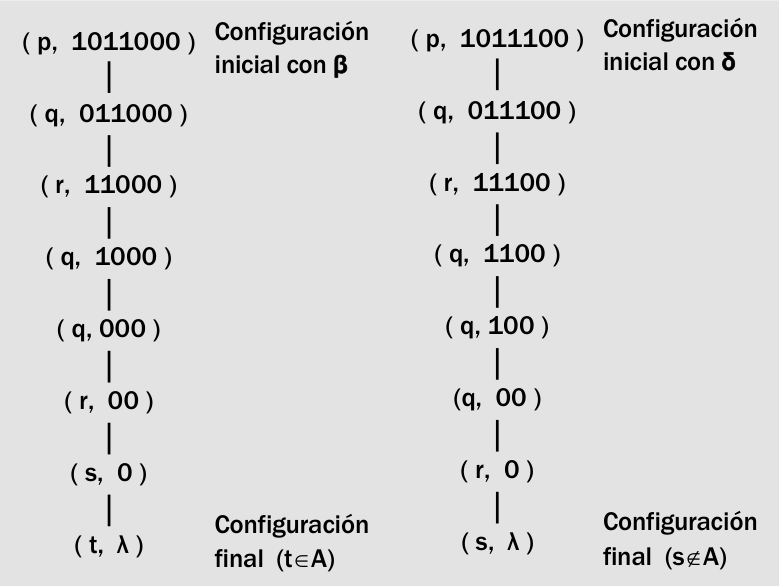
\includegraphics[width=0.5\linewidth]{imagenes/arbol_afd.png}
  \caption{Árboles de descripciones instantáneas}
  \label{fig:arbol_afd}
\end{figure}

\subsubsection{Función de transición extendida}
La función de transición $ f $ define el próximo estado en un $ AFD $ para cada estado actual y ante la entrada de cada posible símbolo. La función de transición extendida $ f^{e}:Q\times \Sigma_{E}^{*} \to Q $ recibe una cadena en vez de un símbolo, y devuelve el último estado en el que se encontrará el $ AFD $ luego de haber leído y haber pasado por cada estado para cada una de las letras de la cadena. Supongamos que $ \alpha=abcde $ pertenece al lenguaje reconocido por el $ AFD $, podemos definir un proceso recursivo que finaliza al completarse la lectura de $ \alpha $:
\[
f^{e}(q,\alpha) = f(f(f(f(f(q,a),b),c),d),e)
\]

\subsubsection{Aceptación de cadenas y otros conceptos asociados a los AFD}
Se dice que un lenguaje $ L $ es aceptado por un autómata finito $ M $ si todas las palabras que lo componene conducen al autómata a estados de aceptación. En símbolos:
\[
L(M) = \left\{\alpha / \alpha \in \Sigma_{E}^{*} \land f^{e}(q_{0},\alpha) \in A\right\}
\]

\subsubsection{Accesibilidad entre estados}
En un $ AFD $, se dice que un estado $ p $ es accesible desde otro estado $ q $, y se representa $ pAq $, si existe una palabra de símbolos de entrada que haga transitar al autómata desde el estado $ q $ hasta el estado $ p $. En símbolos:
\[
pAq  \iff  \exists \alpha \in \Sigma_{E}^{*} / f^{e}(q,\alpha)=p\qquad ,p,q \in Q
\]
Se lee como \textit{$ p $ es accesible desde $ q $ sí y solo sí existe una cadena $ \alpha $ formada por símbolos del alfabeto de entrada tal que, partiendo desde $ q $ y usando una función de transición extendida sobre $ \alpha $, obtenga como resultado $ p $, siendo $ p $ y $ q $ dos estados del conjunto de estados del autómata.}

\subsubsection{Autómatas conexos}
Si todos los estados de un autómata son accesibles desde su estado inicial se dice que el mismo es \textit{conexo}.

\subsubsection{Equivalencia entre estados}
Dos estados $ p,q \in Q $ de un $ AFD $ son equivalentes, y se representa $ pEq $, si desde cualquiera de llos se aceptan y rechazan exactamente las mismas cadenas de símbolos de entrada.
\[
pEq \iff \left[ \forall \alpha \in \Sigma_{E}^{*}: f^{e}(p,\alpha) \in A \iff f^{e}(q,\alpha) \in A\right]
\]

\subsubsection{Equivalencia de longitud entre estados}
Dos estados $ p,q \in Q $ de un $ AFD $ son equivalentes de longitud $ k $, que se representa como $ pEkq $, si son equivalentes para todas las cadenas de largo menor o igual $ k $.
\[
pEq \iff \left[ \forall \alpha \in \Sigma_{E}^{*}: \left|\alpha\right|\leq k \land f^{e}(p,\alpha) \in A \iff f^{e}(q,\alpha) \in A\right]
\]

\subsubsection{Equivalencia entre autómatas}
Dos $ AFD $ $ A_{1} $ y $ A_{2} $ son equivalentes, y se representa $ A_{1}EA_{2} $ si ambos aceptan las mismas palabras o sentencias.
\[
A_{1}EA_{2} \iff L(A_{1}) = L(A_{2})
\]

\subsubsection{Conjunto cociente}
Como toda relación de equivalencía, la relación $ E $ definida sobre el conjunto de estados posibles $ Q $, induce en el mismo una partición. Todos los elementos de $ Q $ relacionados con cierto estado $ p \in Q $, constituyen un subconjunto de $ Q $ que es denominado clase de equivalencia de $ p $. El conjunto cociente es esa partición y se denota $ Q/E $.

La definición de equivalencia entre estados no sirve para saber si dos estados $ p,q \in Q $ son equivalentes, ya que hay infinitas cadenas $ \alpha \in \Sigma_{E}^{*} $. Sin embargo, con el concepto de equivalencia de longitud $ k $ entre estados, es teóricamente posible saber si dos estados $ p,q \in Q $ son $ k $-equivalentes ya que hay un número finito de cadenas $ \alpha \in \Sigma_{E}^{*} $ con $ \left|\alpha\right|\leq k $.

Para encontrar el conjunto cociente podemos usar un procedimiento que consiste en ir buscando equivalencias de longitud $ k $ entre estados comenzando con $ k=0 $ hasta que las clases de equivalencia de $ Q $ se estabilicen.

En el caso de $ AFD_{R} $, el conjunto cociente con $ k=0 $ es:
\[
Q/E_{0} = P_{1}^{0} \cup P_{2}^{0}\qquad ,P_{1}^{0} = Q-A, P_{2}^{0}=A
\]

Los siguientes conjuntos cocientes $ Q/E_{k+1} $ se definen dividiendo las clases $ P_{i}^{k} $ de $ Q/E_{k} $ las veces que sea necesario hasta que, para todo símbolo $ a \in \Sigma_{E} $ y para todo par de estados $ p,q $ de las clases $ P_{i}^{k} $, queden definidos movimientos que conduzcan a elementos de las mismas clases $ Q/E_{k+1} $. Esto se repite hasta obtener $ Q/E_{k+1} = Q/E_{k} $.

\subsubsection{Minimización de autómatas}
Un autómata mínimo es un autómata conexo que cumple correctamente su función con la menor cantidad posible de estados.

Para minimizar un autómata usamos el concepto del conjunto cociente. El autómata mínimo equivalente a uno dado tendrá como estados a cada una de las clases de estados equivalentes del autómata original.

Ejemplo:

Se desea reconocer cadenas que responden al patrón $ (a+b)^{*}ba $ y para ello se propone el siguiente $ AFD $:
\begin{center}
\begin{tikzpicture}[automata]
\node[state, initial, , yshift=0cm, xshift=0cm] (p) {$p$};
\node[state, , right of=p, yshift=1.5cm, xshift=0cm] (q) {$q$};
\node[state, , right of=p, yshift=-1.5cm, xshift=0cm] (r) {$r$};
\node[state, , right of=q, yshift=0cm, xshift=0cm] (s) {$s$};
\node[state, , right of=s, yshift=0cm, xshift=0cm] (t) {$t$};
\node[state, , right of=r, yshift=0cm, xshift=0cm] (v) {$v$};
\node[state, accepting, right of=v, yshift=0cm, xshift=0cm] (u) {$u$};
\draw   (p) edge[above, ] node{a} (q)
	(p) edge[below, ] node{b} (r)
	(q) edge[above, ] node{a} (s)
	(q) edge[above, bend left] node{b} (t)
	(s) edge[left, loop, in=270, out=225, looseness=5] node{a} (s)
	(s) edge[above, ] node{b} (t)
	(t) edge[below, ] node{b} (v)
	(t) edge[left, bend left] node{a} (u)
	(u) edge[right, bend left] node{b} (t)
	(u) edge[above, ] node{a} (s)
	(r) edge[below, ] node{b} (v)
	(r) edge[below, bend right] node{a} (u)
	(v) edge[left, loop, in=90, out=135, looseness=5] node{b} (v)
	(v) edge[below, ] node{a} (u)
;
\end{tikzpicture}
\end{center}

La idea es ahora minimizar este autómata.

Vemos que es conexo, así que podemos comenzar con la minimización, buscando las particiones.

La primera partición del conjunto de estados se obtiene separando a los estados de aceptación del resto, que sería el conjunto cociente para los estados de equivalencia de longitud $ k=0 $ (todas las cadenas reconocidas por el autómata llegan a los estados de aceptación, mientras que las no reconocidas no llegan):
\[
Q/E_{0} = \left\{\left\{p,q,r,s,t,v\right\},\left\{u\right\}\right\}
\]

Lo que podemos hacer ahora es ir nombrando a los subconjuntos de las clases de equivalencia de longitud $ k_{n} $ que vayamos obteniendo para facilitar el proceso de busqueda del conjunto cociente. Entonces podemos decir que para $ k=0 $ tenemos dos subconjuntos $ A=\left\{p,q,r,s,t,v\right\} $ y $ B=\left\{u\right\} $ y juntos forman el conjunto cociente para $ k=0 $: 
\[
Q/E_{0}=\left\{A, B\right\} = \left\{\left\{p,q,r,s,t,v\right\},\left\{u\right\}\right\}
\]

En el siguiente esquema se puede ver gráficamente el proceso de redistribución de los estados equivalentes en los subconjuntos existentes y la incorporación de otros subconjuntos nuevos:
\begin{center}
	\begin{tikzpicture}
		\node (p) {$ p $};
		\node [below of=p] (q) {$ q $};
		\node [below of=q] (r) {$ r $};
		\node [below of=r] (s) {$ s $};
		\node [below of=s] (t) {$ t $};
		\node [below of=t] (v) {$ v $};
		\node [below of=v] (u) {$ u $};

		\node[fit=(p) (q) (r) (s) (t) (v)] (g1) {};
		\draw [decorate, decoration={brace, amplitude=5pt}] (g1.north east) -- (g1.south east);
		\draw [decorate, decoration={brace, amplitude=5pt, mirror}] (g1.north west) -- (g1.south west);

		\draw [decorate, decoration={brace, amplitude=5pt}] (u.north east) -- (u.south east);
		\draw [decorate, decoration={brace, amplitude=5pt, mirror}] (u.north west) -- (u.south west);

		\node [fit=(g1) (u)] (g) {};
		\draw [decorate, decoration={brace, amplitude=5pt, raise=5pt}] (g.north east) -- (g.south east);
		\draw [decorate, decoration={brace, amplitude=5pt, mirror, raise=5pt}] (g.north west) -- (g.south west);


		\node [right of=p, xshift=4cm] (p1) {$ p $};
		\node [below of=p1] (q1) {$ q $};
		\node [below of=q1] (r1) {$ r $};
		\node [below of=r1] (s1) {$ s $};
		\node [below of=s1] (t1) {$ t $};
		\node [below of=t1] (v1) {$ v $};
		\node [below of=v1] (u1) {$ u $};

		\node[fit=(p1) (q1) (r1) (s1) (t1) (v1)] (g11) {};
		\draw [decorate, decoration={brace, amplitude=5pt}] (g11.north east) -- (g11.south east);
		\draw [decorate, decoration={brace, amplitude=5pt, mirror}] (g11.north west) -- (g11.south west);

		\draw [decorate, decoration={brace, amplitude=5pt}] (u1.north east) -- (u1.south east);
		\draw [decorate, decoration={brace, amplitude=5pt, mirror}] (u1.north west) -- (u1.south west);

		\node [fit=(g11) (u1)] (g2) {};
		\draw [decorate, decoration={brace, amplitude=5pt, raise=5pt}] (g2.north east) -- (g2.south east);
		\draw [decorate, decoration={brace, amplitude=5pt, mirror, raise=5pt}] (g2.north west) -- (g2.south west);

		% Flechas rojas
		\draw [->, draw=red, thick] (p) edge[, ] node{} (q1);
		\draw [->, draw=red, thick] (q) edge[, ] node{} (s1);
		\draw [->, draw=red, thick] (r) edge[, ] node{} (u1);
		\draw [->, draw=red, thick] (s) edge[, ] node{} (s1);
		\draw [->, draw=red, thick] (t) edge[, ] node{} (u1);
		\draw [->, draw=red, thick] (v) edge[, ] node{} (u1);
		\draw [->, draw=red, thick] (u) edge[, ] node{} (s1);
		% Flechas azules
		\draw [->, draw=blue, thick] (p) edge[, ] node{} (r1);
		\draw [->, draw=blue, thick] (q) edge[, ] node{} (t1);
		\draw [->, draw=blue, thick] (r) edge[, ] node{} (v1);
		\draw [->, draw=blue, thick] (s) edge[, ] node{} (t1);
		\draw [->, draw=blue, thick] (t) edge[, ] node{} (v1);
		\draw [->, draw=blue, thick] (v) edge[, ] node{} (v1);
		\draw [->, draw=blue, thick] (u) edge[, ] node{} (t1);
		
		% Flechas de la leyenda
		\node [below of=u, xshift=1cm] (leyendaA0) {};
		\node [right of=leyendaA0] (leyendaA1) {};
		\draw [->, draw=red, thick] (leyendaA0) edge[above, ] node{a} (leyendaA1);
		\node [right of=leyendaA1] (leyendaB0) {};
		\node [right of=leyendaB0] (leyendaB1) {};
		\draw [->, draw=blue, thick] (leyendaB0) edge[above, ] node{b} (leyendaB1);


	\end{tikzpicture}
\end{center}

Vemos en el esquema que corresponde a $ k=1 $, que los estados $ p $, $ q $ y $ s $ tienen el mismo comportamiento ya que permanecen los 3 en la clase de equivalencia que se encontraban para todos los símbolos del alfabeto de entrada. Es decir, que no importa el símbolo de entrada que reciba el autómata, los estados $ p $, $ q $ y $ s $ siguen perteneciendo a la clase de equivalencia que habíamos nombrado como $ A $.

Por el contraio, los estados $ r $, $ t $ y $ v $ tienen una conducta común pero diferente a la de los otros estados: ante la entrada $ a $ transitan a la clase de equivalencia $ B $, mientras que con la entrada $ b $ permanecen en la misma clase $ A $. Esto significa que los seis estados de la primera clase no son todos equivalentes con $ k=1 $, por lo que deben ser agrupados en dos subonjuntos diferentes:
\[
Q/E_{1}=\left\{\left\{p,q,s\right\},\left\{r,t,v\right\},\left\{u\right\}\right\}
\]

Otra vez, conviene nombrar a los subconjuntos para que el proceso sea mas facil. De esta forma, podemos nombrar un subconjunto $ A = \left\{p,q,s\right\} $, otro $ B = \left\{r,t,v\right\} $ y por último $ C = \left\{u\right\} $, de manera que:
\[
Q/E_{1} = \left\{A,B,C\right\} = \left\{\left\{p,q,s\right\},\left\{r,t,v\right\},\left\{u\right\}\right\}
\]

La segunda clase de $ Q/E_{0} $ tiene un solo estado $ u $ por lo que no es necesario un análisis.

El siguiente paso es repetir el procedimiento cuando se lee un nuevo símbolo, lo que implica buscar las clases de equivalencia para $ k=2 $. El esquema ahora es el siguiente:
\begin{center}
\begin{tikzpicture}
	\node[, yshift=0cm, xshift=0cm] (p) {$p$};
	\node[below of=p, yshift=0cm, xshift=0cm] (q) {$q$};
	\node[below of=q, yshift=0cm, xshift=0cm] (s) {$s$};
	\node[below of=s, yshift=0cm, xshift=0cm] (r) {$r$};
	\node[below of=r, yshift=0cm, xshift=0cm] (t) {$t$};
	\node[below of=t, yshift=0cm, xshift=0cm] (v) {$v$};
	\node[below of=v, yshift=0cm, xshift=0cm] (u) {$u$};

	\node[fit=(p) (q) (s)] (A) {};
	\draw [decorate, decoration={brace, amplitude=5pt}] (A.north east) -- (A.south east);
	\draw [decorate, decoration={brace, amplitude=5pt, mirror}] (A.north west) -- (A.south west);
	
	\node[fit=(r) (t) (v)] (B) {};
	\draw [decorate, decoration={brace, amplitude=5pt}] (B.north east) -- (B.south east);
	\draw [decorate, decoration={brace, amplitude=5pt, mirror}] (B.north west) -- (B.south west);

	\node[fit=(u)] (C) {};
	\draw [decorate, decoration={brace, amplitude=5pt}] (C.north east) -- (C.south east);
	\draw [decorate, decoration={brace, amplitude=5pt, mirror}] (C.north west) -- (C.south west);

	\node[fit=(A) (B) (C)] (G) {};
	\draw [decorate, decoration={brace, amplitude=5pt, raise=5pt}] (G.north east) -- (G.south east);
	\draw [decorate, decoration={brace, amplitude=5pt, mirror, raise=5pt}] (G.north west) -- (G.south west);

	\node[right of=p, yshift=0cm, xshift=4cm] (p1) {$p$};
	\node[below of=p1, yshift=0cm, xshift=0cm] (q1) {$q$};
	\node[below of=q1, yshift=0cm, xshift=0cm] (s1) {$s$};
	\node[below of=s1, yshift=0cm, xshift=0cm] (r1) {$r$};
	\node[below of=r1, yshift=0cm, xshift=0cm] (t1) {$t$};
	\node[below of=t1, yshift=0cm, xshift=0cm] (v1) {$v$};
	\node[below of=v1, yshift=0cm, xshift=0cm] (u1) {$u$};

	\node[fit=(p1) (q1) (s1)] (A) {};
	\draw [decorate, decoration={brace, amplitude=5pt}] (A.north east) -- (A.south east);
	\draw [decorate, decoration={brace, amplitude=5pt, mirror}] (A.north west) -- (A.south west);
	
	\node[fit=(r1) (t1) (v1)] (B) {};
	\draw [decorate, decoration={brace, amplitude=5pt}] (B.north east) -- (B.south east);
	\draw [decorate, decoration={brace, amplitude=5pt, mirror}] (B.north west) -- (B.south west);

	\node[fit=(u1)] (C) {};
	\draw [decorate, decoration={brace, amplitude=5pt}] (C.north east) -- (C.south east);
	\draw [decorate, decoration={brace, amplitude=5pt, mirror}] (C.north west) -- (C.south west);

	\node[fit=(A) (B) (C)] (G) {};
	\draw [decorate, decoration={brace, amplitude=5pt, raise=5pt}] (G.north east) -- (G.south east);
	\draw [decorate, decoration={brace, amplitude=5pt, mirror, raise=5pt}] (G.north west) -- (G.south west);
	
	\draw [->, draw=red, thick] (p) edge[, ] node{} (q1);
	\draw [->, draw=red, thick] (q) edge[, ] node{} (s1);
	\draw [->, draw=red, thick] (s) edge[, ] node{} (s1);
	\draw [->, draw=red, thick] (r) edge[, ] node{} (u1);
	\draw [->, draw=red, thick] (t) edge[, ] node{} (u1);
	\draw [->, draw=red, thick] (v) edge[, ] node{} (u1);
	\draw [->, draw=red, thick] (u) edge[, ] node{} (s1);

	\draw [->, draw=blue, thick] (p) edge[, ] node{} (r1);
	\draw [->, draw=blue, thick] (q) edge[, ] node{} (t1);
	\draw [->, draw=blue, thick] (s) edge[, ] node{} (t1);
	\draw [->, draw=blue, thick] (r) edge[, ] node{} (v1);
	\draw [->, draw=blue, thick] (t) edge[, ] node{} (v1);
	\draw [->, draw=blue, thick] (v) edge[, ] node{} (v1);
	\draw [->, draw=blue, thick] (u) edge[, ] node{} (t1);
	
\end{tikzpicture}
\end{center}

Ahora podemos ver que al analizar las clases de equivalencia para $ k=2 $ los estados agrupados en cada subconjunto mantienen su equivalencia entre sí:
\begin{itemize}
  \item Para la entrada $ a $, los estados $ p $, $ q $ y $ s $ transitan a la clase $ B $. Y para la entrada $ b $, se quedan en la clase $ A $.

  \item Para la entrada $ a $, los estados $ r $, $ t $ y $ v $ transitan a la clase $ C $. Y para la entrada $ b $, se quedan en la clase $ B $.

  \item En el conjunto $ C $ solo hay un elemento por lo que no es necesario su análisis.
\end{itemize}

Esto significa que el conjunto cociente se estabilizó y no va a cambiar si seguimos analizando $ k $ mayores a 2. De esta manera, el conjunto cociente $ Q/E $ es el que acabamos de encontrar:
\[
Q/E_{2} = \left\{\left\{p,q,s\right\},\left\{r,t,v\right\},\left\{u\right\}\right\} = Q/E_{1} = Q/E
\]

Y si usamos los nombres que le habíamos asignado a cada subconjunto, podemos decir que:
\[
Q/E = \left\{A,B,C\right\}
\]

Acá me confundí: No debería haber usado la letra $ A $ para nombrar un subconjunto ya que vamos a ver que al definir al autómata formalmente, este se puede confundir con el estado de aceptación que también tiene por nombre $ A $. No lo voy a cambiar porque ya me dió paja, y creo que igual se entiende lo que hicimos y tampoco es tan confusa la definición formal siguiente. Solo hay que tener en cuenta que el $ A \in Q $ no es el estado de aceptación y son dos cosas distintas.

El $ AFD $ mínimo tiene la siguiente definición formal:
\[
AFD = \left(\Sigma_{E},Q,q_{0},A,f\right)
\]
donde:
\begin{align*}
  \Sigma_{E} &= \left\{a,b\right\}\\
  Q &= \left\{A,B,C\right\}\\
  q_{0} &= A\\
  A &= C\\
  f &= \left\{((A,a),A),((A,b),B),((B,a),C),((B,b),B),((C,a),A),((C,b),B)\right\}
\end{align*}

Sabemos que el estado $ q_{0} = A $ porque el autómata original empezaba en el estado $ p \in A $. También sabemos que el estado de aceptación es $ A = C $ porque el autómata original terminaba en el estado $ u \in C $.

El dígrafo del $ AFD $ es el siguiente:
\begin{center}
\begin{tikzpicture}[automata]
\node[state, initial, , yshift=0cm, xshift=0cm] (A) {$A$};
\node[state, , right of=A, yshift=0cm, xshift=0cm] (B) {$B$};
\node[state, accepting, right of=B, yshift=0cm, xshift=0cm] (C) {$C$};

\draw   (A) edge[left, loop below] node{a} (A)
	(A) edge[above, ] node{b} (B)
	(B) edge[left, loop below] node{b} (B)
	(B) edge[above, ] node{a} (C)
	(C) edge[below, bend left] node{b} (B)
	(C) edge[above, bend right] node{a} (A)
;
\end{tikzpicture}
\end{center}

\subsection{Autómatatas Finitos Bidireccionales}
Los autómatas finitos leen siempre la cadena de entrada de izquierda a derecha. Esto tiene varias consecuencias:
\begin{itemize}
  \item Cada símbolo de la cadena es leído una única vez.

  \item Al completarse la lectura, la cadena es aceptada o no, según se alcance un estado de aceptación.

  \item La cantidad de intervalos de tiempo necesarios para evaluar la cadea es igual a su largo.

  \item En todo momento está claramente definida la subcadena pendiente de ser leída.
\end{itemize}

Si le otorgamos a un $ AFD $ la capacidad de decidir el sentido del movimiento del cabezal en cada intervalo de tiempo tenemos un \textbf{Autómata Finito Determinista Bidireccional (AFDB)}. A la definición del autómata entonces, se le debe incorporar una \textit{función de movimiento} que defina el sentido del movimiento del cabezal en cada estado y ante cada símbolo de entrada. También hay que definir el sector de la cinta en el que el autómata debe operar, y para esto se incorporan dos símbolos especiales que indican el inicio y el fin del intervalo de la cinta de entrada a ser analizado.

\subsubsection{Características del AFDB}
\begin{itemize}
  \item Cada símbolo de entrada puede ser leído varias veces.

  \item No hay ninguna condición que indique el fin de la lectura de la cadena.

  \item No es posible anticipar la cantidad de intervalos de tiempo requeridos para evaluar la cadena.

  \item El concepto de cadena que resta de ser leída desaparece.
\end{itemize}

\subsubsection{Definición de un AFDB}
El $ AFDB $ se define como:
\[
AFDB = \left(\Sigma_{E},\Gamma,Q,q_{0},A,f\right)
\]
donde:
\begin{align*}
  \Sigma_{E} &: \text{Alfabeto de símbolos de entrada}\\
  \Gamma &: \text{Alfabeto de cinta,} && \Gamma=\Sigma_{E} \cup \left\{ \vdash, \dashv  \right\}\\
  Q &: \text{Conjunto finito, no vacío, de estados posibles}\\
  q_{0} &: \text{Estado inicial de operación,} && q_{0} \in Q\\
  A &: \text{Conjunto de estados de aceptación,} && A \subseteq Q\\
  f &: \text{Función de transición,} && f:Q\times \Gamma \to Q\times \left\{I,N,D\right\}
\end{align*}
donde $ I,N,D $ significan izquierda, neutro y derecha respectivamente.

\subsubsection{Aceptación de cadenas}
Una cadena es aceptada por el $ AFDB $ cuando éste ha alcanzado un estado de aceptación y la cadena ha sido leída por lo menos una vez. En otras palabras, la cantidad de intervalos de tiempo requeridos para la aceptación de una cadena es igual o mayor que su largo.

\subsubsection{Configuración o descripción instantánea}
Para definir la condición en la que se encuentra un $ AFDB $ en un instante dado se requieren tres componentes:
\begin{itemize}
  \item El estado actual.

  \item El contenido de la cinta de entrada.

  \item La posición del cabezal.
\end{itemize}

Para la posición del cabezal la convención indica que el símbolo de inicio de cinta $  \vdash  $ está en la posición $ 0 $, y el contador se incrementa hacia la derecha, lo que implica que el primer caracter de la cadena de entrada está en la posición $ 1 $.

Según este criterio, la configuración $ K_{t} $ de un $ AFDB $ que opera sobre una cierta cadena de entrada $ \alpha $, que en el instante $ t $ está en el estado $ q $ y con el cabezal en la posición $ k $ es:
\[
K_{t} = (q,  \vdash \alpha  \dashv , k)
\]

Esto nos permite saber el estado en el que se encuentra el autómata en un tiempo $ t $, vemos la cadena que tiene que procesar el autómata, y con la posición del cabezal vemos qué símbolo de esa cadena está procesando el autómata.

La configuración inicial es entonces:
\[
K_{0} = (q_{0}, \vdash \alpha \dashv ,0)
\]
y la configuración final de aceptación es:
\[
K_{A} = (q_{A},  \vdash \alpha \dashv ,n) \quad ,q_{A} \in A,n=\left|\alpha\right|+1
\]

Otra forma de representar la configuración de un $ AFDB $ es:
\[
K_{t} = \delta q\beta
\]

Donde $ q $ es el estado actual del atómata, $ \delta $ el prefijo de la cadena de entrada $ \alpha $ que antecede al cabezal y $ \beta $ el sufijo que sigue al cabezal $ (\alpha=\delta\beta) $. Según este criterio, la configuración inicial es $ K_{0}=q_{0}\alpha $ y la final es $ K_{A}=\alpha q_{A} $.

Por ejemplo, si $ \alpha=abcdef $ y el autómata leyó el caracter $ b $, la configuración sería $ K_{2}=abq_{0}cdef $.

\subsubsection{Lenguaje reconocido por el AFDB}
Se puede definir el lenguaje $ L $ reconocido por el $ AFDB $ $ M $ como:
\[
L(M) = \left\{\alpha / \alpha \in \Sigma_{E}^{*} \land q_{0}\alpha \mapsto ^{*}\alpha q_{A}\quad ,q_{a} \in A\right\}
\]

Que se lee como \textit{el lenguaje $ L $ reconocido por el autómata $ M $ son todas las cadenas que se puedan formar con el alfabeto de entrada que, empezando desde el estado inicial, se puedan procesar para llegar al estado de aceptación}.

\subsubsection{Equivalencia entre AFDB y AFD}
El movimiento del caberzal en dos sentidos no brinda ninguna capacidad adicional con respecto al $ AFD $, lo que implicax que todo $ AFDB $ tiene un $ AFD $ equivalente.

\section{Autómata Finito No Determinista (AFND)}
Como ya habíamos dicho, un autómata finito deja de ser determinista cuando su función de transición no es una función. Es decir, si un $ AF $ en un cierto estado y ante una cierta señal de entrada admite multiples estados, este es un \textbf{Autómata Finito No Determinista (AFND)}. Al igual que en el caso de los $ AFD $, los $ AFND $ quedan definidos como una quíntupla:
\[
AFND = \left(\Sigma_{E},Q,q_{0},A,f\right)
\]
solo que en este caso, la función de transición es en realidad una relación de transición y queda definida de la siguiente forma:
\[
f:Q\times \Sigma_{E} \to \mathcal{P}(Q) 
\]
donde $ \mathcal{P}(Q) $ es el conjunto potencia de $ Q $.

En los $ AFND $ es díficil saber cuánto tiempo va a llevar el procesamiento de una cadena debido a que para cada estado pueden existir múltiples caminos a tomar. El tiempo demandado para resolver este tipo de problemas es exponencial, lo que implica un esfuerzo muy considerable incluso para casos simples.

Por otro lado, el diseño de estos autómatas es mas sencillo que el de los $ AFD $ por lo que el no determinismo de los autómatas resulta de gran ayuda para el diseño de autómatas destinados a reconocer lenguajes complejos, pagando el costo de un mayor esfuerzo de operación.

Ejemplo: Analicemos el siguiente $ AFND $ destinado a reconocer cadenas del siguiente tipo $ \alpha=(0+1)^{*}1000 $.
\begin{center}
\begin{tikzpicture}[automata]
\node[state, initial, , yshift=0cm, xshift=0cm] (p) {$p$};
\node[state, , right of=p, yshift=0cm, xshift=0cm] (q) {$q$};
\node[state, , right of=q, yshift=0cm, xshift=0cm] (r) {$r$};
\node[state, , right of=r, yshift=0cm, xshift=0cm] (s) {$s$};
\node[state, accepting, right of=s, yshift=0cm, xshift=0cm] (t) {$t$};

\draw   (p) edge[above, loop above] node{0,1} (p)
	(p) edge[above, ] node{1} (q)
	(q) edge[above, ] node{0} (r)
	(r) edge[above, ] node{0} (s)
	(s) edge[above, ] node{0} (t)
;
\end{tikzpicture}
\end{center}

Podemos ver que este autómata es no determinista ya que en el estado $ p $, para la entrada $ 1 $ se puede ir a mas de un estado.

Si le pasamos al $ AFND $ la cadena $ \beta=1011000 $ puede comprobarse que el éste acepta la cadena al arribar al estado $ t $, pero para ello tuvo que explorar varias opciones que podemos ver en las siguientes figuras que corresponden al \textit{árbol de descripciones instantáneas} y al \textit{plano estados-entradas}.

\begin{figure}[H]
  \centering
  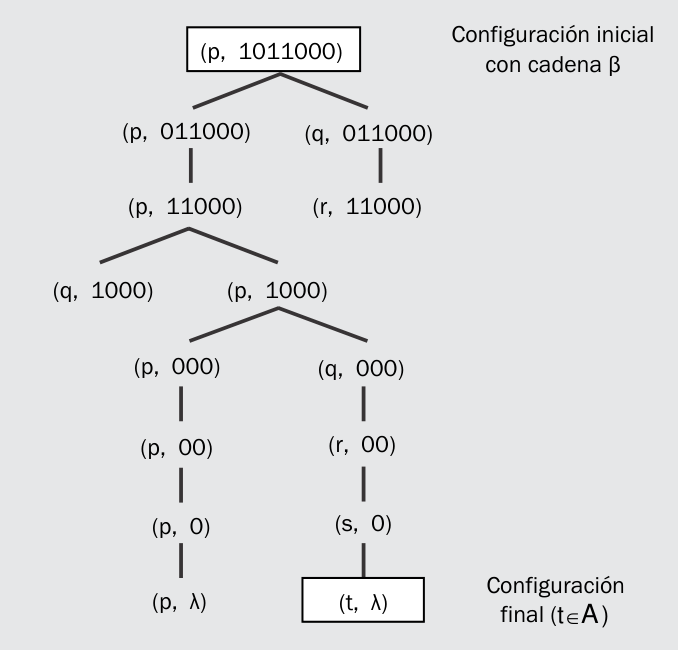
\includegraphics[width=0.5\linewidth]{imagenes/arbol_afnd.png}
  \caption{Árbol de descripciones instantáneas.}
  \label{fig:arbol_afnd}
\end{figure}
\begin{figure}[H]
  \centering
  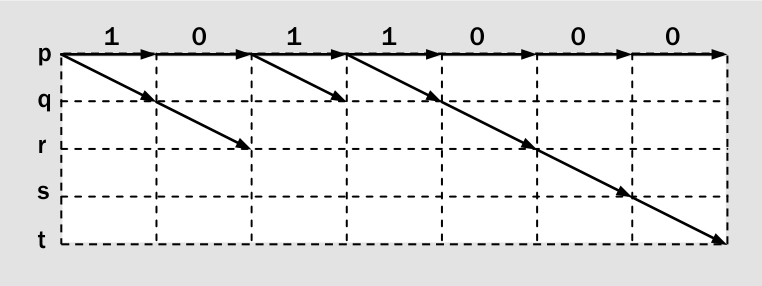
\includegraphics[width=0.5\linewidth]{imagenes/plano_afnd.png}
  \caption{Representación del plano estados-entradas.}
  \label{fig:plano_afnd}
\end{figure}

Podemos ver que en 2 oportunidades el $ AFND $ no pudo continuar operando con la cadena entrada ya que no existían transiciones que lo permitan cuando lee $ 1 $ en los estados $ q $ o $ r $. También vemos que en otras dos oportunidades el autómata sí leyó la cadena completa, pero en un caso llegó al estado $ p $ que no es de aceptación, y en el otro llegó al estado $ t $ que sí es de aceptación y es esta la razón por la que la cadena fue aceptada.

\subsection{Transiciónes Lambda}
La definición de los $ AFND $ puede ampliarse para incluir transiciones de un estado a otro que no dependan de ninguna entrada, y son denominadas \textbf{transiciones $ \lambda $}. Estos autómatas se denominan $ AFND-\lambda $.

En estos casos, $ \lambda $ pasa a ser un nuevo símbolo del alfabeto de entrada. De esta manera, hay que reescribir la relación de transición $ f $ para incluir el símbolo $ \lambda $ al alfabeto de entrada y considerar los pares $ (q,\lambda) $. Ademas se asume que cada estado tiene su propia transición $ \lambda $ que cicla sobre sí mismo:
\[
f:Q\times (\Sigma_{E} \cup \left\{\lambda\right\}) \to \mathcal{P}(Q)
\]

A todos los pares de estados que están relacionados por una transición $ \lambda $ los podemos agrupar en un conjunto $ T $ denomindao \textit{relación de transición $ \lambda $}.
\[
T=\underbrace{\left\{(p,q) / q \in f(p,\lambda)\right\}}_{\text{Todos los $ p $ y $ q $ relacionados con $ \lambda $}} \cup \underbrace{\left\{(q,q) / q \in Q\right\}}_{\text{Todos los $ q $ tienen su ciclo con $ \lambda $}}
\]

Luego se incorporan al conjunto $ T $ TODOS los pares ordenados que se originan de la propiedad transitiva de los pares anteriores:
\[
T^{*} = T \cup \left\{(p,r) / pTq \land qTr\right\}
\]

\subsection{Lambda-clausura}
Se denomina $ \lambda \text{{\textminus}}clausura(p)$ al conjunto de todos los estados $ q \in Q $ que están relacionados con $ p $ por medio del cierre transitivo de de la relación de transición $ \lambda $ ($ T^{*} $). En símbolos:
\[
	\lambda \text{{\textminus}} clausura(p) = \left\{q \in Q / (p,q) \in T^{*}\right\}
\]

Ejemplo: Supongamos que tenemos el siguiente $ AFND\text{{\textminus}}\lambda $ y queremos obtener la $ \lambda\text{{\textminus}}clausura $ de todos sus estados:
\begin{center}
\begin{tikzpicture}[automata]
\node[state, initial, , yshift=0cm, xshift=0cm] (p) {$p$};
\node[state, , right of=p, yshift=0cm, xshift=0cm] (q) {$q$};
\node[state, accepting, right of=q, yshift=0cm, xshift=0cm] (r) {$r$};

\draw   (p) edge[above, loop above] node{0} (p)
	(p) edge[above, ] node{$ \lambda $} (q)
	(q) edge[above, loop above] node{1} (q)
	(q) edge[above, ] node{$ \lambda $} (r)
	(r) edge[above, loop above] node{2} (r)
;
\end{tikzpicture}
\end{center}

Para armar la $ \lambda\text{{\textminus}}clausura $ necesitamos tener $ T^{*} $, pero para eso necesitamos primero obtener $ T $, que son todas las tuplas $ (p,q) $ relacionadas por $ \lambda $ y todas las tuplas $ (q,q) $ ya que siempre cada estado se puede relacionar con sigo mismo por medio de $ \lambda $.
\[
T=\left\{(p,q),(q,r),(p,p),(q,q),(r,r)\right\}
\]

Ahora, a $ T $ le agregamos todos los pares ordenados que originan de la propiedad transitiva de los pares ordenados de $ T $:
\[
T^{*}=\left\{(p,q),(q,r),(p,p),(q,q),(r,r),(p,r)\right\}
\]

Y ahora sí, podemos buscar la $ \lambda\text{{\textminus}}clausura $ para cada uno de los estados del $ AFND\text{{\textminus}}\lambda $:
\begin{align*}
  \lambda\text{{\textminus}}clausura(p) &= \left\{p,q,r\right\}\\
  \lambda\text{{\textminus}}clausura(q) &= \left\{r,q\right\}\\
  \lambda\text{{\textminus}}clausura(r) &= \left\{r\right\}
\end{align*}

\subsection{Equivalencia con autómatas finitos deterministas}
Para la equivalencia entre autómatas fínitos existen dos teoremas.
\subsubsection{Teorema 1: AFND-lambda a AFND}

Sea un $ AFND-\lambda $ que es definido como $ M = (\Sigma_{E},Q,q_{0},A,f) $ donde
\[
f:Q\times (\Sigma_{E} \cup \left\{\lambda\right\}) \to \mathcal{P}(Q) 
\]

Este autómata puede siempre ser redefinido como un $ AFND $ en el que $ M^{\prime} = (\Sigma_{E},Q,q_{0},A^{\prime},f^{\prime}) $ donde $ f^{\prime}:Q\times \Sigma_{E} \to \mathcal{P}(Q)  $ siguiendo los siguientes pasos:
\begin{enumerate}[a)]
  \item Obtenemos la $ \lambda\text{{\textminus}}clausura(q),\forall q \in Q $ de todos los estados $ q $ del autómata.

  \item Para cada estado $ q \in Q $, armamos un conjunto con $ f(p,a) $, siendo $ p \in \lambda\text{{\textminus}}clausura(q) $ cada estado de la $ \lambda\text{{\textminus}}clausura(q) $ y $ a \in \Sigma_{E} $ un símbolo del alfabeto de entrada. También unimos a este conjunto, el conjunto $ \lambda\text{{\textminus}}clausura(p) $ para todo $ p $ cuya relación $ f(p,a) $ esté definida.

	  El conjunto para cada estado $ q \in Q $ quedaría así:
	  \[
		  q_{a} = \left\{f(p,a)\right\} \cup \left\{f(p,a) \in Q \implies \lambda\text{{\textminus}}clausura(p)\right\}
	  \]

  \item Repetimos el paso anterior para cada símbolo $ a \in \Sigma_{E} $ del alfabeto de entrada.

  \item Si en $ \lambda\text{{\textminus}}clausura(q_{0}) $ se encuentra algún estado final $ q_{A} $, entonces el conjunto de estados finales del nuevo autómata es $ A \cup \left\{q_{0}\right\} $, de lo contrario el conjunto de estados finales $ A $ no se vé modificado. 

  \item El estado inicial del nuevo autómata es el mismo que el estado inicial del $ AFND\text{{\textminus}}\lambda $.

  \item Reescribimos el autómata usando los conjuntos que armamos recién como si fuesen las relaciones de transición.
\end{enumerate}

Ejemplo: Queremos convertir el $ AFND\text{{\textminus}}\lambda $ del ejemplo anterior en un $ AFND $ equivalente:

\begin{center}
\begin{tikzpicture}[automata]
\node[state, initial, , yshift=0cm, xshift=0cm] (p) {$p$};
\node[state, , right of=p, yshift=0cm, xshift=0cm] (q) {$q$};
\node[state, accepting, right of=q, yshift=0cm, xshift=0cm] (r) {$r$};

\draw   (p) edge[above, loop above] node{0} (p)
	(p) edge[above, ] node{$ \lambda $} (q)
	(q) edge[above, loop above] node{1} (q)
	(q) edge[above, ] node{$ \lambda $} (r)
	(r) edge[above, loop above] node{2} (r)
;
\end{tikzpicture}
\end{center}

\begin{enumerate}[a)]
  \item Ya habíamos definido los $ \lambda\text{{\textminus}}clausura $ de cada estado:
	\begin{align*}
	  \lambda\text{{\textminus}}clausura(p) &= \left\{p,q,r\right\}\\
	  \lambda\text{{\textminus}}clausura(q) &= \left\{r,q\right\}\\
	  \lambda\text{{\textminus}}clausura(r) &= \left\{r\right\}
	\end{align*}

  \item \begin{align*}
    p_{0} &= \left\{p\right\} \cup \left\{p,q,r\right\} = \left\{p,q,r\right\}\\
    q_{0} &=  \varnothing \\
    r_{0} &=  \varnothing 
  \end{align*}

  \item Repetimos el punto anterior para el resto de símbolos del afabeto de entrada:
	  \begin{align*}
	    p_{1} &= \left\{q\right\} \cup \left\{q,r\right\} = \left\{q,r\right\}\\
	    q_{1} &= \left\{q\right\} \cup \left\{q,r\right\} = \left\{q,r\right\}\\
	    r_{1} &=  \varnothing \\
	    p_{2} &= \left\{r\right\} \cup \left\{r\right\} = \left\{r\right\}\\
	    q_{2} &= \left\{r\right\} \cup \left\{r\right\} = \left\{r\right\}\\
	    r_{2} &= \left\{r\right\} \cup \left\{r\right\} = \left\{r\right\}
	  \end{align*}

  \item $ q,r,s \in A $ son los tres un estado de aceptación ya que todos tienen a $ r $ en su $ \lambda\text{{\textminus}}clausura $.

  \item El estado inicial sigue siendo $ p $.

  \item Reescribimos el autómata como un $ AFND $:

	  \begin{center}
	  \begin{tikzpicture}[automata]
	  \node[state, initial, accepting, yshift=0cm, xshift=0cm] (p) {$p$};
	  \node[state, , right of=p, yshift=0cm, xshift=0cm] (q) {$q$};
	  \node[state, accepting, right of=q, yshift=0cm, xshift=0cm] (r) {$r$};

	  \draw   (p) edge[above, loop above] node{0} (p)
		  (p) edge[above, ] node{0,1} (q)
		  (p) edge[below, bend right] node{0,1,2} (r)
		  (q) edge[above, loop above] node{1} (q)
		  (q) edge[above, ] node{1,2} (r)
		  (r) edge[above, loop above] node{2} (r)
	  ;
	  \end{tikzpicture}
	  \end{center}
\end{enumerate}

\subsubsection{Teorema 2: AFND a AFD}

Sea un $ AFND $ definido como $ M=(\Sigma_{E},Q,q_{0},A,f) $ donde
\[
f:Q\times \Sigma_{E} \to \mathcal{P}(Q) 
\]

Siempre se puede encontrar un $ AFD $ $ M^{\prime}=(\Sigma_{E},Q^{\prime},c_{0},A^{\prime},f^{\prime}) $ con $ f:Q\times \Sigma_{E} \to Q^{\prime} $ que es equivalente siguiendo estos pasos:
\begin{enumerate}[a)]
  \item Reconocemos el estado inicial del $ AFND $ y lo nombramos como $ c_{0} $.

  \item Por cada símbolo $ a \in \Sigma_{E} $ buscamos un nuevo conjunto $ c_{i+1}=f(q,a) $ siendo $ q $ todos los estados que pertenecen a $ c_{i} $.

  \item Repetimos el paso anterior hasta que no encontremos mas conjuntos nuevos.

  \item El estado inicial del $ AFD $ equivalente es el mismo que el $ AFND $.

  \item El conjunto de estados finales del $ AFD $ es el conjunto de estados finales $ A $ unión todos los $ c_{i} $ que contengan al menos un estado final en ellos. En símbolos: $ A^{\prime}=c_{i} \in Q^{\prime} / c_{i} \cap A\neq  \varnothing  $.

  \item Podemos graficar el $ AFD $ equivalente sabiendo que cada $ c_{i} $ encontrado es un estado del mismo.
\end{enumerate}

Ejemplo: Queremos convertir el siguiente $ AFND $ en un $ AFD $ equivalente:
\begin{center}
\begin{tikzpicture}[automata]
\node[state, initial, accepting, yshift=0cm, xshift=0cm] (p) {$p$};
\node[state, , right of=p, yshift=0cm, xshift=0cm] (q) {$q$};
\node[state, accepting, right of=q, yshift=0cm, xshift=0cm] (r) {$r$};

\draw   (p) edge[above, loop above] node{0} (p)
	(p) edge[above, bend left] node{0} (q)
	(q) edge[above, loop above] node{0} (q)
	(q) edge[above, bend left] node{1} (r)
	(q) edge[above, bend left] node{0} (p)
	(r) edge[above, loop above] node{1} (r)
	(r) edge[above, bend left] node{0} (q)
;
\end{tikzpicture}
\end{center}

\begin{enumerate}[a)]
  \item El estado inicial es:
	  \[
		  c_{0}=\left\{p\right\}
	  \]

  \item Buscamos nuevos conjuntos $ c_{i} $: 
  \begin{align*}
    f(c_{0},0) &= \left\{p,q\right\} = c_{1} && \text{Le asignamos un nombre porque encontramos un conjunto nuevo}\\
    f(c_{0},1) &=  \varnothing && \text{Como es vacio no hacemos nada}
  \end{align*}

  \item En el paso anterior encontramos al menos un conjunto nuevo, así que analizamos ese conjunto:
  \begin{align*}
    f(c_{1},0) &= \left\{p,q\right\}  \cup \left\{p,q\right\} && \text{Es igual a $ c_{1} $ así que no hacemos nada}\\
    f(c_{1},1) &=  \varnothing  \cup \left\{r\right\} = c_{2} && \text{Le asignamos un nombre porque es un conjunto nuevo}\\
    f(c_{2},0) &= \left\{q\right\} = c_{3} && \text{Le asignamos un nombre porque es un conjunto nuevo}\\
    f(c_{2},1) &= \left\{r\right\} && \text{Es igual a $ c_{2} $ así que no hacemos nada}\\
    f(c_{3},0) &= \left\{p,q\right\} &&  \text{Es igual a $ c_{1} $ así que no hacemos nada}\\
    f(c_{3},1) &= \left\{r\right\} && \text{Es igual a $ c_{2} $ así que no hacemos nada}
  \end{align*}

  \item Ya no encontramos mas estados nuevos así que no repetimos mas. El estado inicial de nuestro $ AFD $ es $ c_{0} $.

  \item Los estados finales del $ AFND $ eran $ p $ y $ r $ así que todos los $ c_{i} $ que contengan a $ p $ o $ r $ van a ser estados finales del $ AFD $. En este caso los estados finales son: $ c_{0} $, $ c_{1} $ y $ c_{2} $

  \item Ahora podemos graficar nuestro $ AFD $:
	\begin{center}
	\begin{tikzpicture}[automata]
	\node[state, initial, accepting, yshift=0cm, xshift=0cm] (c0) {$c_{0}$};
	\node[state, accepting, right of=c0, yshift=2cm, xshift=0cm] (c1) {$c_{1}$};
	\node[state, accepting, right of=c1, yshift=-2cm, xshift=0cm] (c2) {$c_{2}$};
	\node[state, , right of=c0, yshift=-2cm, xshift=0cm] (c3) {$c_{3}$};

	\draw   (c0) edge[above, bend left] node{0} (c1)
		(c1) edge[above, loop above] node{0} (c1)
		(c1) edge[above, bend left] node{1} (c2)
		(c2) edge[below, bend left] node{0} (c3)
		(c2) edge[above, loop right] node{1} (c2)
		(c3) edge[left, bend left] node{0} (c1)
		(c3) edge[below, bend left] node{1} (c2)
	;
	\end{tikzpicture}
	\end{center}
\end{enumerate}

\subsection{Gramáticas regulares y autómatas finitos}
Hasta ahora veníamos creando los autómatas a base de prueba y error. Pero, en realidad es posible crearlos sistemáticamente a partir de reglas de producción de las gramáticas. A su vez, también es posible definir las reglas de producción capaces de generar lenguajes a ser reconocidos por ciertos autómatas.

\subsubsection{Definición de gramáticas regulares a partir de autómatas}
La idea es definir el conjunto de reglas de producción de una gramática regular que generará lenguajes que están destinados a ser reconocidos por un cierto $ AFD $. La gramática que vamos a obtener va a estar bien formada y será lineal por derecha.

\fbox{\parbox{0.9\linewidth}{
\textbf{}

Dado un $ AFD = (\Sigma,Q,q_{0},A,f) $, la gramática que genera el mismo lenguaje que acepta el autómata sera $ G=(\Sigma,Q,q_{0},P) $, donde el conjunto de reglas de reescritura queda definido como:
\[
P=\left\{X:=aY / f(X,a)=Y\right\} \cup \left\{X:=a / f(X,a)=Y,Y \in A\right\}
\]
y se agrega $ q_{0}:=\lambda $ si $ q_{0} \in A $; $ \quad X,Y,q_{0} \in Q,a \in \Sigma,A \subseteq Q $
}}\vspace{0.2cm}

Ejemplo: Determinar la gramática bien formada capaz de generar las sentencias  del lenguaje reconocido por el siguiente $ AFD $:
\begin{center}
\begin{tikzpicture}[automata]
\node[state, initial, , yshift=0cm, xshift=0cm] (p) {$p$};
\node[state, , right of=p, yshift=0cm, xshift=0cm] (q) {$q$};
\node[state, , right of=q, yshift=0cm, xshift=0cm] (r) {$r$};
\node[state, , right of=r, yshift=0cm, xshift=0cm] (s) {$s$};
\node[state, accepting, right of=s, yshift=0cm, xshift=0cm] (t) {$t$};

\draw   (p) edge[above, loop above] node{0} (p)
	(p) edge[above, ] node{1} (q)
	(q) edge[above, bend left] node{0} (r)
	(q) edge[above, loop above] node{1} (q)
	(r) edge[above, bend left] node{0} (s)
	(r) edge[above, bend left=40] node{1} (q)
	(s) edge[above, bend left] node{0} (t)
	(s) edge[above, bend left=50] node{1} (q)
	(t) edge[above, bend right=45] node{0} (p)
	(t) edge[above, bend left=60] node{1} (q)
;
\end{tikzpicture}
\end{center}

Convertimos las transiciones en reglas de producción según lo que se explica en el cuadro anterior:
\[
\left.
\begin{aligned}
  f(p,0) &= p\\
  f(p,1) &= q\\
  f(q,0) &= r\\
  f(q,1) &= q\\
  f(r,0) &= s\\
  f(r,1) &= q\\
  f(s,0) &= t\\
  f(s,1) &= q\\
  f(t,0) &= p\\
  f(t,1) &= q
\end{aligned}
\right\} \implies 
\left\{
\begin{aligned}
  p &:= 0p\\
  p &:= 1q\\
  q &:= 0r\\
  q &:= 1q\\
  r &:= 0s\\
  r &:= 1q\\
  s &:= 0t \mid 0\\
  s &:= 1q\\
  t &:= 0p\\
  t &:= 1q
\end{aligned}
\right.
\]

No hay que olvidarse de agregar los $ X:=a $ cuando $ f(X,a)=B,B \in A $, como se hizo con el estado $ s $.

El conjunto completo de las reglas de producción de la gramática es entonces:
\[
P = 
\left\{
\begin{aligned}
	p &:= 0p \mid 1q,\\
	q &:= 0r \mid 1q,\\
	r &:= 0s \mid 1q,\\
	s &:= 0t \mid 1q \mid 0,\\
	t &:= 0p \mid 1q
\end{aligned}
\right\}
\]

Y la gramática que buscabamos es:
\[
G=\left(\left\{0,1\right\},\left\{p,q,r,s,t\right\},p,P\right)
\]

\subsubsection{Definición de autómatas a partir de gramáticas regulares}
En este caso ya conocemos la gramática, que estará bien formada y será lineal por derecha, y lo que queremos hacer es definir el autómata que es capaz de reconocer el lenguaje generado.

\fbox{\parbox{0.9\linewidth}{
\textbf{}

Dada la gramática regular $ G=(\Sigma_{T},\Sigma_{N},S,P) $, el autómata finito que acepta el mismo lenguaje que genera la gramática será:
\[
AF=(\Sigma_{T},\Sigma_{N} \cup \left\{A\right\},S,\left\{A\right\},f)
\]
donde $ A $ es un nuevo símbolo que no estaba en $ \Sigma_{N} $, $ f(X,a)=Y $ si $ X:=aY $ está en $ P $, y $ f(X,a)=A $ si $ X:=a $ está en $ P $, con $ X,Y,S \in \Sigma_{N},a \in \Sigma_{T} $.

La regla de producción $ S:=\lambda $ incropora la transición $ f(S,\lambda)=A $.
}}\vspace{0.2cm}

\textbf{Nota}: Si la gramática es lineal por izquierda, es necesario convertirla previamente a lineal por derecha, aplicando el procedimiento adecuado.

Ejemplo: Definir en $ AFD $ que reconozca el lenguaje generado por la siguiente gramática lineal por derecha:
\[
G=\left(\left\{a,b\right\},\left\{p,q,r,s,t\right\},p,P\right)
\]
donde 
\[
P = 
\left\{
\begin{aligned}
	p &:= 0p \mid 1q,\\
	q &:= 0r \mid 1q,\\
	r &:= 0s \mid 1q,\\
	s &:= 0t \mid 1q \mid 0,\\
	t &:= 0p \mid 1q
\end{aligned}
\right\}
\]

Según el procedimiento explicado para las gramáticas bien formadas, a cada producción $ X:=aY $ le corresponde una transición $ f(X,a)=Y $. Entonces tenemos que:
\[
\begin{aligned}
	f(p,0) &= p & f(p,1) &= q\\
	f(q,0) &= r & f(q,1) &= q\\
	f(r,0) &= s & f(r,1) &= q\\
	f(s,0) &= t & f(s,1) &= q\\
	f(t,0) &= p & f(t,1) &= q
\end{aligned}
\]

En este caso, $ p $ resulta ser el estado inicial $ q_{0}=p $ por ser $ p $ el axioma. La regla de producción $ s:=0 $ indica que hay que agregar $ f(s,0)=A $ y sabemos que $ f(s,0)=t $, por lo tanto $ t \in A $.

Con la información que tenemos podemos ya armar el autómata que es el siguiente:
\begin{center}
\begin{tikzpicture}[automata]
\node[state, initial, , yshift=0cm, xshift=0cm] (p) {$p$};
\node[state, , right of=p, yshift=0cm, xshift=0cm] (q) {$q$};
\node[state, , right of=q, yshift=0cm, xshift=0cm] (r) {$r$};
\node[state, , right of=r, yshift=0cm, xshift=0cm] (s) {$s$};
\node[state, accepting, right of=s, yshift=0cm, xshift=0cm] (t) {$t$};

\draw   (p) edge[above, loop above] node{0} (p)
	(p) edge[above, ] node{1} (q)
	(q) edge[above, bend left] node{0} (r)
	(q) edge[above, loop above] node{1} (q)
	(r) edge[above, bend left] node{0} (s)
	(r) edge[above, bend left=40] node{1} (q)
	(s) edge[above, bend left] node{0} (t)
	(s) edge[above, bend left=50] node{1} (q)
	(t) edge[above, bend right=45] node{0} (p)
	(t) edge[above, bend left=60] node{1} (q)
;
\end{tikzpicture}
\end{center}


\subsubsection{Conversión de gramática lineal por izquierda a lineal por derecha}
Para cada gramática lineal por izquierda existe una gramática lineal por derecha y viceversa. Para realizar esta conversión hay que seguir los siguientes cuatro pasos:

\paragraph{Paso 1}\mbox{}: Si la gramática es recursiva en el axioma hay que convertirla a otra equivalente que no sea recursiva en el axioma. Para ello hay que incorporar un nuevo símbolo no terminal $ B $ y modificar las reglas de producción de la siguiente manera:
\begin{itemize}
  \item Por cada regla $ S:=\alpha $, se crea una nueva regla $ B:=\alpha $.

  \item Cada regla de la forma $ A:=Sa $ debe ser reemplazada por $ A:=Ba $, donde $ S,A,B \in \Sigma_{N}, a \in \Sigma_{T} $ y $ \alpha $ es una cadena válida.
\end{itemize}

\paragraph{Paso 2}\mbox{}: Se debe construir un grafo con las siguientes instrucciones:
\begin{itemize}
  \item Los nodos del grafo se identifican con los símbolos no terminales de la gramática y se incluye un nodo adicional identificado con $ \lambda $.

  \item Por cada regla de la forma $ A:=Ba $, se dibuja una arista desde el nodo $ A $ al nodo $ B $ que es identificado con la etiqueta $ a $.

  \item Por cada regla de la forma $ A:=a $, se dibuja una arista dese el nodo $ A $ al nodo $ \lambda $ identificado con $ a $.

  \item Para la regla $ S:=\lambda $, se incorpora una arista sin etiqueta desde el nodo $ S $ al nodo $ \lambda $.
\end{itemize}

\paragraph{Paso 3}\mbox{}: Se construye un nuevo grafo a partir del grafo anterior según se indica:
\begin{itemize}
  \item Se intercambian los identificadores de los nodos $ S $ y $ \lambda $.

  \item Se cambia el sentido de todas las aristas.
\end{itemize}

\paragraph{Paso 4}\mbox{}: A partir del nuevo grafo, se obtiene la gramática lineal por derecha siguiendo los siguientes pasos:
\begin{itemize}
  \item Los alfabetos de símbolos terminales y no terminales son los mismo de la gramática original lineal por izquierda.

  \item Por cada arista dirigida etiquetada con $ a $ desde el nodo $ B $ al nodo $ A $, se incorpora a la nueva gramática la regla de producción $ B:=aA $.

  \item Por cada arista dirigida etiquetada con $ a $ desde el nodo $ B $ al nodo $ \lambda $, se incorpora la regla de producción $ B;=a $.

  \item En caso de una arista sin etiqueta desde el nodo $ S $ al nodo $ \lambda $, se incorpora a la gramática la regla $ S:=\lambda $.
\end{itemize}

Ejemplo: La siguiente gramática $ G $ que es lineal por izquierda debe ser convertida en lineal por derecha para poder definir el $ AFD $ que reconoce el lenguaje generado por ella.
\[
G=\left(\left\{0,1,2\right\},\left\{X,Y,Z\right\},X,P\right)
\]
\[
P=\left\{X:=Z0 \mid Y0 \mid 0 \mid 1,Y:=Y0 \mid 1,Z:=Z2 \mid 2\right\}
\]

Seguimos los pasos descriptos anteriormente:
\begin{enumerate}[1.]
  \item La gramática no es recursiva en el axioma así que no tenemos que hacer nada en este paso.

  \item Realizamos el grafo:
	  \begin{center}
	  \begin{tikzpicture}[automata]
	  \node[state, , yshift=0cm, xshift=0cm] (x) {$X$};
	  \node[state, , right of=x, yshift=0cm, xshift=0cm] (y) {$Y$};
	  \node[state, , right of=y, yshift=0cm, xshift=0cm] (z) {$Z$};
	  \node[state, , right of=z, yshift=0cm, xshift=0cm] (lamda) {$\lambda$};

	  \draw   (x) edge[below, bend right] node{0} (z)
		  (x) edge[above, ] node{0} (y)
		  (x) edge[below, bend right=40] node{0,1} (lamda)
		  (y) edge[above, loop above] node{0} (y)
		  (y) edge[above, bend left] node{1} (lamda)
		  (z) edge[above, loop below] node{2} (z)
		  (z) edge[above, ] node{2} (lamda)
	  ;
	  \end{tikzpicture}
	  \end{center}

  \item Modificamos el grafo anterior:
	  \begin{center}
	  \begin{tikzpicture}[automata]
	  \node[state, , yshift=0cm, xshift=0cm] (x) {$\lambda$};
	  \node[state, , right of=x, yshift=0cm, xshift=0cm] (y) {$Y$};
	  \node[state, , right of=y, yshift=0cm, xshift=0cm] (z) {$Z$};
	  \node[state, , right of=z, yshift=0cm, xshift=0cm] (lamda) {$X$};

	  \draw   (z) edge[above, bend right] node{0} (x)
		  (y) edge[above, ] node{0} (x)
		  (lamda) edge[above, bend right=40] node{0,1} (x)
		  (y) edge[above, loop below] node{0} (y)
		  (lamda) edge[below, bend left] node{1} (y)
		  (z) edge[above, loop above] node{2} (z)
		  (lamda) edge[above, ] node{2} (z)
	  ;
	  \end{tikzpicture}
	  \end{center}

  \item \begin{itemize}
    \item Los alfabetos de símbolos terminales y no terminales son los mismos de antes.

    \item Las primeras reglas de producción que se crean son las siguientes: $ X:=2Z \mid 1Y, Z:=2Z,Y:=0Y $.

    \item Las siguientes reglas de producción que se crean son estas: $ X:=0 \mid 1, Z:=0, Y:=0 $.

    \item No hay aristas sin etiquetas.
  \end{itemize}
\end{enumerate}

De esta forma, la gramática obtenida es la siguiente:
\[
G=\left(\left\{0,1,2\right\},\left\{X,Y,Z\right\},X,P\right)
\]
\[
P=\left\{X:=2Z \mid 1Y \mid 0 \mid 1,Y:=0Y \mid 0,Z:=2Z \mid 0\right\}
\]

\subsection{Expresiones regulares y autómatas finitos}
Lo que se va a presentar ahora es un algorítmo que permite construir para cada expresión regular, un $ AFND\text{{\textminus}}\lambda $ que reconozca el mismo lenguaje descripto por ella.

\subsubsection{Algorítmo de Thompson}
El algorítmo de Thompson traduce cada parte de una expresión regular en un atómata que acepta el mismo lenguaje denotado por ella.
A continuación vamos item por item de la definición de una expresión regular y graficamos el autómata equivalente.

La definición la podemos ver de nuevo en esta sección \ref{sec:regex}.
\begin{enumerate}[a)]
  \item Autómata equivalente a $  \varnothing  $:
	  \begin{center}
	  \begin{tikzpicture}[automata]
	  \node[state, initial, , yshift=0cm, xshift=0cm] (p) {$q_{0}$};
	  \node[state, accepting, right of=p, yshift=0cm, xshift=0cm] (q) {$q_{A}$};
	  \end{tikzpicture}
	  \end{center}

  \item Autómata equivalente a $ \lambda $:
	  \begin{center}
	  \begin{tikzpicture}[automata]
	  \node[state, initial, , yshift=0cm, xshift=0cm] (p) {$q_{0}$};
	  \node[state, accepting, right of=p, yshift=0cm, xshift=0cm] (q) {$q_{A}$};
	  \draw   (p) edge[above, ] node{$ \lambda $} (q)
	  ;
	  \end{tikzpicture}
	  \end{center}

  \item Autómata equivalente a la expresión $ a $:
	  \begin{center}
	  \begin{tikzpicture}[automata]
	  \node[state, initial, , yshift=0cm, xshift=0cm] (p) {$q_{0}$};
	  \node[state, accepting, right of=p, yshift=0cm, xshift=0cm] (q) {$q_{A}$};
	  \draw   (p) edge[above, ] node{a} (q)
	  ;
	  \end{tikzpicture}
	  \end{center}

	  Ahora suponemos los que los autómatas $ AF_{E} $ y $ AF_{F} $ que reconocen las expresiones regulares $ E $ y $ F $ ya existen.

  \item Autómata equivalente a $ E+F $, notar que se quitan los estados de inicio y aceptacion de los automatas $ AF_{E} $ y $ AF_{F} $:
	  \begin{center}
	  \begin{tikzpicture}[automata]
	  \node[state, initial, , yshift=0cm, xshift=0cm] (q0) {$q_{0}$};
	  \node[state, , right of=q0, yshift=2cm, xshift=0cm] (e0) {$q_{0E}$};
	  \node[state, , right of=e0, yshift=0cm, xshift=0cm] (ea) {$q_{AE}$};
	  \node[state, , right of=q0, yshift=-2cm, xshift=0cm] (f0) {$q_{0F}$};
	  \node[state, , right of=f0, yshift=0cm, xshift=0cm] (fa) {$q_{AF}$};
	  \node[state, accepting, right of=fa, yshift=2cm, xshift=0cm] (qa) {$q_{A}$};
	  \node[fit=(e0) (ea),draw] (afe) {};
	  \node[fit=(f0) (fa),draw] (aff) {};
	  \draw   (e0) edge[above, ] node{E} (ea)
		  (f0) edge[above, ] node{F} (fa)
		  (q0) edge[above, bend left=20] node{$ \lambda $} (afe)
		  (q0) edge[below, bend right=20] node{$ \lambda $} (aff)
		  (afe) edge[above, bend left=20] node{$ \lambda $} (qa)
		  (aff) edge[below, bend right=20] node{$ \lambda $} (qa)
	  ;
	  \end{tikzpicture}
	  \end{center}

  \item Autómata equivalente a $ EF $, se quitan los estados de inicio y aceptación de $ AF_{E} $ y $ AF_{F} $:
	  \begin{center}
	  \begin{tikzpicture}[automata]
	  \node[state, initial, , yshift=0cm, xshift=0cm] (q0) {$q_{0}$};
	  \node[state, , right of=q0, yshift=0cm, xshift=0cm] (e0) {$q_{0E}$};
	  \node[state, , right of=e0, yshift=0cm, xshift=0cm] (ea) {$q_{AE}$};
	  \node[state, , right of=e0, yshift=-3cm, xshift=0cm] (f0) {$q_{0F}$};
	  \node[state, , right of=f0, yshift=0cm, xshift=0cm] (fa) {$q_{AF}$};
	  \node[state, accepting, right of=fa, yshift=0cm, xshift=0cm] (qa) {$q_{A}$};
	  \node[fit=(e0) (ea),draw] (afe) {};
	  \node[fit=(f0) (fa),draw] (aff) {};
	  \draw   (e0) edge[above, ] node{E} (ea)
		  (f0) edge[above, ] node{F} (fa)
		  (q0) edge[above, ] node{$ \lambda $} (afe)
		  (afe) edge[above, out=0, in=180, looseness=5] node{$ \lambda $} (aff)
		  (aff) edge[above, ] node{$ \lambda $} (qa)
	  ;
	  \end{tikzpicture}
	  \end{center}
	  \newpage

  \item Autómata equivalente a $ E^{*} $, se quitan los estados de inicio y aceptación de $ AF_{E} $:
	  \begin{center}
	  \begin{tikzpicture}[automata]
	  \node[state, initial, , yshift=0cm, xshift=0cm] (q0) {$q_{0}$};
	  \node[state, , right of=q0, yshift=0cm, xshift=0cm] (e0) {$q_{0E}$};
	  \node[state, , right of=e0, yshift=0cm, xshift=0cm] (ea) {$q_{AE}$};
	  \node[state, accepting, right of=ea, yshift=0cm, xshift=0cm] (qa) {$q_{A}$};
	  \node[fit=(e0) (ea),draw] (afe) {};
	  \draw   (e0) edge[above, ] node{E} (ea)
		  (q0) edge[above, ] node{$ \lambda $} (afe)
		  (afe) edge[above, ] node{$ \lambda $} (qa)
		  (q0) edge[below, bend right] node{$ \lambda $} (qa)
		  (afe) edge[above, loop above, out=30, in=150, looseness=2] node{$ \lambda $} (afe)
	  ;
	  \end{tikzpicture}
	  \end{center}
\end{enumerate}

El algorítmo de Thompson termina construyendo un $ AFND\text{{\textminus}}\lambda $ con muchos estados, por lo que debe ser luego transformado en $ AFD $ y posiblemente minimizado para que sea eficiente su implementación, pero es muy útil ya que todos estos procesos son automáticos y pueden ser programados (es lo que hace el generador de analizadores léxicos \textit{lex} de UNIX).


%\addcontentsline{toc}{section}{Referencias}
%\printbibliography

\end{document}
